\documentclass[12pt,titlepage]{article}

%% THE USEPACKAGES NECESSARY FOR THIS EXAMPLE
%% NOTE THAT genetics_manu_style MUST BE CALLED AFTER mychicago
\usepackage{graphicx}
\usepackage{endfloat}
\usepackage{amsfonts}
\usepackage{subfigure}
\usepackage{genetics_manu_style}

\usepackage{siunitx}
\sisetup{output-exponent-marker=\ensuremath{\mathrm{E}}}

% Add hyperlinks
%\usepackage{hyperref}

% amsmath package, useful for mathematical formulas
\usepackage{amsmath}
% amssymb package, useful for mathematical symbols
\usepackage{amssymb}

% graphicx package, useful for including eps and pdf graphics
% include graphics with the command \includegraphics
\usepackage{graphicx}

% cite package, to clean up citations in the main text. Do not remove.
%\usepackage{cite}
\usepackage{natbib}
\bibpunct{(}{)}{;}{author-year}{}{,} 

\usepackage[dvipsnames]{xcolor}

% Use doublespacing - comment out for single spacing
\usepackage{setspace}

% For splitting/combining figures.
\usepackage{subfigure}

% Use doublespacing - comment out for single spacing
%\usepackage{setspace} 
%\doublespacing

% Split table cells
%\usepackage{slashbox}

% Table with curly braces
\usepackage{multirow,bigdelim}

% Underline 
\usepackage[normalem]{ulem}


\newcommand{\St}{\mathcal{S}}
\newcommand{\It}{\mathcal{I}}
\newcommand{\Rt}{\mathcal{R}}
\newcommand{\traj}{\mathcal{V}}

\newcommand{\tree}{\mathcal{T}}

\newcommand{\comment}[1]{{\color{red} (#1)}}
\newcommand{\ajd}[1]{{\color{black} #1}}

\newcommand{\stochCoalSIR}{stochastic coalescent SIR}
\newcommand{\deterCoalSIR}{deterministic coalescent SIR}

\newcommand{\StochCoalSIR}{Stoch. Coal. SIR}
\newcommand{\DeterCoalSIR}{Deter. Coal. SIR}


\newcommand{\stochSIR}{stochastic SIR}
\newcommand{\StochSIR}{Stochastic SIR}
\newcommand{\BDSIR}{BDSIR}

%TANJA: Do we say somewhere what priors we use in the BDSIR for psi/(mu+psi). I wonder if we misspecify there a bit and thus are different from coalescent methods in the HIV data analysis. ( the R0 value inferred by coalescent is high indicating that the methods might produce similar results....). Just to make clear: I'm not saying we should do more analyses here, simply trying to understand what we did...

%% THE MANUSCRIPT TITLE
%\title{\LARGE{Stochasticity and determinism in coalescent SIR: Bayesian epidemic inference}\\
\title{\LARGE{Bayesian Coalescent Epidemic Inference:  Comparison of Stochastic and Deterministic SIR Population Dynamics}\\
\vspace{10mm}}


%%  THE AUTHOR DECLARATIONS.  USE \THANKS TO GIVE ADDRESSES
\author{Alex Popinga\thanks{Department of Computer Science, University of Auckland, Auckland, New Zealand 1010}\thanks{Allan Wilson Centre for Molecular Ecology and Evolution, New Zealand PN4442},  
Tim Vaughan$^{\ast}$$^{\dag}$\thanks{Massey University, Palmerston North, New Zealand 4442}, 
Tanja Stadler\thanks{Department of Biosystems Science and Engineering, ETH Z\"urich, Basel, Switzerland}, 
Alexei J Drummond$^{\ast}$$^{\dag}$}

%% USE \RENEWCOMMAND FOR CORRESPONDING ADDRESS, RUNNING HEAD
%% AND KEYWORDS, ETC.
\renewcommand{\CorrespondingAddress}{Department of Computer Science \\
    University of Auckland \\ 
    303 - 379\\
    38 Princes St\\ 
    Auckland, NZ 1010 \\ 
    (64 9) 373-7599 88298 \\
    %\texttt{alexpopinga@gmail.com} \vfill}
    \texttt{alexei@cs.auckland.ac.nz} \vfill}
\renewcommand{\RunningHead}{Bayesian Coalescent Epidemic Inference}
%\renewcommand{\CorrespondingAuthor}{Alex Popinga, Alexei Drummond}
\renewcommand{\CorrespondingAuthor}{Alexei J Drummond}
\renewcommand{\KeyWords}{Bayesian inference, Phylodynamics, Coalescent, Epidemic, Stochastic} % stop adding keywords! Genetics only accepts 5!

%% SOME COMMANDS FOR THE CONTENT OF THIS FILE.  NOT NECESSARY FOR
%% GENETIC_MANU_STYLE
\newcommand{\bp}{\mathbf{p}}
\newcommand{\LLL}{\mathcal{L}}

%% BEGIN DOC
\begin{document}


\maketitle



%% ABSTRACT ENVIRONMENT
\begin{abstract}

Estimation of epidemiological and population parameters from molecular sequence data has become central to the understanding of infectious disease dynamics.  
Various models have been proposed to infer details of the dynamics that describe epidemic progression. 
These include inference approaches derived from Kingman's coalescent as well as from birth-death branching processes.  
%Concurrently, methods of incorporating additional information into phylogenetic inference have grown increasingly sophisticated. 
The development of alternative approaches merits investigation of their characteristics and differences. 
Here we use recently described coalescent theory for epidemic dynamics to develop stochastic and deterministic coalescent SIR tree priors. We implement these in a Bayesian phylogenetic inference framework to permit joint estimation of SIR epidemic parameters and the sample genealogy. 
We assess the models' performance and contrast results obtained with a recently published birth-death-sampling model for epidemic inference.  
Comparisons are made by analyzing sets of genealogies
simulated under precisely known epidemiological parameters.  
We also compare results of analyses using published HIV-1 sequence data obtained from
known UK infection clusters.  
We show that the coalescent SIR model is effective at estimating epidemiological parameters from data with large fundamental reproductive number $R_0$ and large population size $S_0$. 
We find that the stochastic variant generally outperforms its deterministic counterpart.  However, each of these Bayesian estimators are shown to have undesirable properties in certain circumstances, especially for epidemic outbreaks with $R_0$ close to one or with small susceptible populations.

%TANJA: what about one closing sentence about comparison to the birth-death-sampling model for epidemic inference, as we mention it above?

%We implemented a recent coalescent model for inferring key epidemiological parameters from genetic sequence data into a Bayesian framework 
%for the case of homogeneous host populations. We used the extension additional information embedded in time-stamped (heterochronous) sequence data 
%in the face of genealogical uncertainty.  We compare the performance of these inference methods, conditional on both deterministic and stochastic epidemiological models,
%and contrast the results with those obtained using the recently-published BDSIR method.  Initial comparisons are accomplished first by using sets of genealogies
%simulated under precisely known epidemiological parameters.  Subsequent comparisons are made by analysis of published HIV-1 sequence data obtained from
%known UK infection clusters.  

\end{abstract}


\section{Introduction}

\subsection{Phylodynamics and the coalescent}

The epidemiological and evolutionary processes that underpin rapidly evolving 
species occur on a shared spatiotemporal frame of reference.  Unified analyses 
that include both the dynamics of an epidemic and the reconstruction of the pathogen phylogeny can 
therefore elucidate imperative, and otherwise inaccessible, information to aid in the 
development of vaccines and other methods of outbreak prevention.  Such information 
includes the rates of pathogen transmission and host recovery, effective population sizes 
(e.g., numbers of susceptible and infected individuals), and the `time of origin' representing the 
introduction of the first infected individual into a population of susceptible hosts.

The term \textit{phylodynamics} was popularized by \cite{Grenfell16012004} to describe the interlaced study of immunodynamics, 
epidemiology, and evolutionary mechanisms.  Since then several phylodynamic models, both 
stochastic and deterministic in nature, have been developed to characterize the 
phylogenetic history of the pathogen species and compartmentalizations of the host 
population throughout the epidemic.  Such models grant the ability to infer 
key epidemiological parameters from the genetic sequence data and include birth-death 
branching processes \citep{Stadler:2012,Stadler:2013,Kuhnert:2014,gavryushkina2014bayesian}, as well as 
coalescent approaches \citep{GriffithsandTavare:1994,Pybus22062001, KoelleandRasmussen, Rasmussen2011, DearloveandWilson,Rasmussen2014} derived from 
Kingman's coalescent theory \citep{Kingman:1982}.

A significant step toward the unification of epidemiology and
statistical phylogenetics was made by \cite{Volz:2009}, who formalized
the application of Kingman's $n$-coalescent to pathogen population
dynamics. The original published method involved numerical integration
of a set of ordinary differential equations (ODEs) to find a
deterministic approximation to the variation in the number of sampled
lineages through time. Assuming no correlation between the rates at
which pathogen lineage pairs coalesce, the probability density of a
pathogen genealogy (conditional on the parameters of the
epidemiological model) could then be determined directly from this
ancestor function.  In a subsequent paper, \cite{Volz:2012} dispensed
with this approximation and significantly elaborated on the original
model, extending the tree density calculation to allow for
serially-sampled and spatially structured genetic sequence data.  In
this coalescent model, the birth and death rates can vary in time and
by the state of the host, so that ``the birth rate of a single gene
copy is both time- and state-dependent.''

In this paper, we assess the capability of Bayesian
inference methods centred around the latter class of coalescent-based
phylodynamic models to recover a range of parameters (including the
basic reproduction number) from simulated data.  
While \cite{DearloveandWilson} paved the way by implementing a coalescent approach for deterministic SI, SIS, and SIR models in the Bayesian environment, 
we implement and then rigorously test both extended stochastic and deterministic models of epidemic dynamics.

\subsection{Stochastic and deterministic models}

Stochasticity and determinism each maintain dominant roles in particular stages 
of an epidemic.  Once the infected population has grown considerably large, on the order 
of 1,000 to 10,000 lineages, the probability densities of stochastically expressed 
population size dynamics converge toward the deterministic interpretation \citep{Rouzine:2001}. However, 
during the early stages the population size of infected individuals is small, and the 
dynamics of the epidemic are therefore governed by stochastic processes according to the 
relative significance of fluctuations in the demographic and rate parameters of the 
population model \citep{Kuhnert:2014}.

Population size is critical to the epidemiological system and, as with any parameter in a 
Bayesian setting, yields the most accurate estimations when detailed prior information 
is available and incorporated into the inference \citep{Drummond:2006}.   Even so, 
approximating the prevalence of infection by deterministic interpretation requires the 
number of infected hosts within the effective population to be assumed as very large 
throughout the duration of the described epidemic (i.e., once the exponential growth phase 
has been reached), lest the whole description breaks down \citep{Rouzine:2001}.
%Furthermore, this large-population limit is restricted specifically to the 
%\textit{sampled} genealogies, which may be appreciably smaller still.

In our extension and implementation of the coalescent model for epidemics, both stochastic and deterministic population size
processes are used for the simulation of trees and/or trajectories for subsequent inference.

\subsection{Compartmental population models (SIR)}

Host populations can be compartmentalized simply but effectively in 
mathematical models that describe epidemic progression.  The specific division of the 
aggregate population depends on the nature of the contagion in question, spanning a range 
of scenarios where hosts may or may not be reinfected, possess more than one infection 
rate, exhibit a period of exposure between becoming infected and becoming infectious, and 
so forth.  Such examples cover the well-known SI (Susceptible-Infected), 
SIS (Susceptible-Infected-Susceptible), SIR (Susceptible-Infected-Removed), and SEIR 
(Susceptible-Exposed-Infected-Removed) paradigms \citep{Anderson:1991fk, Keeling:2008zr}.
Each of these compartments can be expressed either
(a) by a set of ordinary differential equations (ODEs) describing the deterministic
time development of real-valued compartment occupancies, or (b) in terms of integer-valued
occupancies governed by continuous-time Markov chains (CTMC) that allow for a degree of
uncertainty in the timing and number of events that occur over the course of the epidemic.

%Currently, the probabilities of phylogenetic trees in both stochastic and deterministic SI and SIS systems can be solved 
%analytically [\cite{Leventhal:2014}], but populations associated with the SIR description 
%must be treated numerically.  

In this paper, we concentrate on the SIR model, which describes epidemics that 
include infected individuals who are at some point in time removed from the effective 
population by way of immunity, death, behavioral changes, or some other cessation of infecting others and being 
reinfected.  
The deterministic variant of this model is given by the trio of coupled
ODEs,
\begin{eqnarray}
\frac{d}{dt} S(t) &=& - \beta I(t)S(t),\label{eq:SIR1}\\
\frac{d}{dt} I(t) &=& \beta I(t)S(t) - \gamma I(t),\label{eq:SIR2}\\
\frac{d}{dt} R(t) &=& \gamma I(t),\label{eq:SIR3}
\end{eqnarray}
%TANJA: shall we say that the model is fully defined with the initial conditions S(0), I(0) and R(0) ? (as we mention the initial conditions also for the stochastic model).
where $\beta$ and $\gamma$ respectively represent the transition rates
from susceptible $S$ to infected $I$, and infected $I$ to removed
$R$. 
\ajd{This deterministic model fully defines the population dynamics with initial conditions $S(0)$, $I(0)$, and $R(0)$, and}
 throughout this paper we refer to solutions to this set of
equations as \emph{deterministic SIR trajectories}.

The comparable stochastic description is given in terms of the probability
of the epidemic state at time $t$ given its initial state and the rate parameters
\begin{equation}
\pi(s,i,r;t) \equiv \Pr(S(t)=s, I(t)=i, R(t)=r|S(0),I(0),R(0),\beta,\gamma),
\end{equation}
which are governed by the following equation of motion:
\begin{align}
\frac{d}{dt}\pi(s,i,r;t)=&\beta\left[(s+1)(i-1)\pi(s+1,i-1,r;t)-si\pi(s,i,r;t)\right]\nonumber\\
&+\gamma\left[(i+1)\pi(s,i+1,r-1;t)-i\pi(s,i,r;t)\right].
\label{eq:SIRME}
\end{align}
An explicit sampling process is incorporated by allowing each removal
event to coincide with a sampling event with a fixed probability
$\psi/(\psi+\mu)$ where $\psi$ and $\mu$ are the overall rates of
sampled and unsampled removals, respectively, such that
$\gamma=\psi+\mu$. We refer to epidemic histories sampled from this
model as \emph{stochastic SIR trajectories}.

Both types of epidemic trajectories can be related to models of sampled transmission tree
genealogies. In the deterministic case, this relationship is made via
the coalescent distributions described in %\cite{Volz:2009} and
\cite{Volz:2012}. We call this the
\emph{deterministic coalescent SIR model}.  In the stochastic case,
genealogies appear naturally from a branching process in which the
branching events coincide with the transmission events in the CTMC and
only those lineages ancestral to sampled removals are recorded. We
call this the \emph{stochastic SIR model}.  The \emph{BDSIR model} introduced by
\cite{Kuhnert:2014} provides an approximation to the stochastic
SIR model.

Another way of relating the stochastic SIR model to sampled
transmission trees involves drawing a realization of a stochastic SIR
epidemic, then using coalescent distribution in \cite{Volz:2012} to
produce a tree conditional on the particular piecewise constant
infected compartment size corresponding to that realization.  We call
this approach the \emph{stochastic coalescent SIR model}.

Both the transmission rate $\beta$ and removal rate $\gamma$ can be
estimated using each of the methods considered in this paper from data
ascribed to an SIR epidemic.

%\noindent{The system is nonlinear and mathematically posits a constant effective population size $N$ by }
%\begin{eqnarray}
%\frac{d}{dt} {S} + \frac{d}{dt} {I} + \frac{d}{dt} {R} &=& 0,
%\end{eqnarray}
%\noindent{and therefore}
%\begin{eqnarray}
%\ \St(\tau) + \It(\tau) + \Rt(\tau) &=& N.
%\end{eqnarray}

%\vspace{5 mm}
%\noindent{\textbf{d) Bayesian implementation}}
%\vspace{3 mm}


\section{Methods}

\subsection{Inference framework}



%We implemented a recently described coalescent SIR model \cite{Volz:2012} in a Bayesian inference framework.

%Although restricted to a single, well-mixed host population, our
% implementation handles uncertainty in the phylogeny and
% serially-sampled data. This is achieved by exploiting the posterior
% probability density,

All phylodynamic inference discussed in this paper is based on the joint posterior probability density
\begin{eqnarray}
\ f(\tree,\traj,\eta, \theta | D) = \frac{\mathbb{P} (D|\tree,\theta) f(\tree|\traj,\eta) f(\traj |\eta) f(\eta) f(\theta) }{\mathbb{P}(D)},
\label{eq:posterior}
\end{eqnarray}
where the (transmission) tree $\tree$, the epidemic trajectory denoted $\traj = \left( \St,\It,\Rt \right)$, the substitution parameters $\theta$, and the epidemiological parameters $\eta = \{\beta,\gamma,S_0,z_0\}$ are all estimated from the sequence data.  
Here $\St$, $\It$, and $\Rt$ represent the host compartment sizes from the present time ($\tau=0$) back to the origin $z_{0}$, units ago:
\begin{eqnarray}
\St(\tau) &=& S(z_{0}-\tau), \\
\It(\tau) &=& I(z_{0}-\tau), \\
\Rt(\tau) &=& R(z_{0}-\tau).  
\end{eqnarray}

The various terms making up the right-hand side of
eq.~(\ref{eq:posterior}) are the tree likelihood
$\mathbb{P}(D|\tree,\theta)$, the tree prior $f(\tree|\traj,\eta)$,
the epidemic trajectory density $f(\traj|\eta)$, and the substitution
and epidemiological parameter priors $f(\eta)$ and $f(\theta)$. (The
probability $\mathbb{P}(D)$ is merely a normalizing constant and can
be ignored.)  It is the product of the tree prior and trajectory
density $f(\tree|\traj,\eta)f(\traj|\eta)$ that distinguishes each of
the models considered in this paper.

% The parameter prior probability $f(\theta)$ summarizes what we know about the parameters before observing the data, and $\mathbb{P}(D)$ is the normalizing constant.  The probability of the sequence data given the tree and substitution model parameter values (calculated with Felsenstein's pruning algorithm \citep{Felsenstein:2004}), and the density of the tree given the epidemic, are represented by the tree likelihood $\mathbb{P}(D|\tree,\theta)$ and the tree prior $f(\tree|\traj,\eta)$, respectively. The form of the probability density of a particular epidemic history given the epidemiological parameters $f(\traj|\eta)$ depends on the particular model of tree generation: the deterministic coalescent SIR, the stochastic coalescent SIR or BDSIR. In the deterministic case, we simply have $f(\traj|\eta)=\delta(\traj-\traj_{\eta})$, where $\traj_{\eta}$ is the single trajectory implied by the parameters.  The densities for the stohastic models are non-singular as each parameter combination supports a variety of individual trajectories.


For both the deterministic and stochastic coalescent SIR models, the tree prior $f(\tree|\traj,\eta)$ is calculated in the following way.  First, consider the time span of a tree divided into segments bracketed by both 
sampling and coalescent events. By considering intervals ending in sampling events as well as coalescent-ending intervals, we follow previous work
that extended coalescent approaches to time-stamped, serially-sampled data \citep{RodrigoFelsenstein1999,Drummond:2002}.
 Interval $i$ is spanned by $k_i$ lineages and is the 
$i$'th interval when ordered from the most recent tip to the root. The set of intervals 
$A$ ending in sample events and the set of intervals $Y$ ending in coalescent events 
together encompass all intervals, $V = A \cup Y$. Let the end time of an interval be $\tau_i$ 
(going back in time), with $\tau_0=0$ as the time of the most recent tip and with time increasing 
into the past. Then the probability density of a genealogy given an epidemic trajectory is
\begin{equation}
f(\tree|\traj, \eta) = \prod_{i \in Y} {\lambda}_{k_{i}}(\tau_i) \prod_{i\in V}\omega(\tau_i, 
k_i),
\label{eq:treeGivenTraj}
\end{equation}
where $\lambda_{k_i}(\tau)$ is the instantaneous coalescent rate at $\tau$ prescribed by
\cite{Volz:2012}
\begin{align}
\lambda_{k_i}(\tau) &= \binom{k_i}{2}\frac{2{\beta}{\St}({\tau})}{{\It}({\tau})},
\label{eq:coalrate}
\end{align}
and where $\omega(\tau_i,k_i)$ is the waiting probability density
\begin{equation}
\omega(\tau_i, k_i) = \exp\left({-{\int_{\tau_{i-1}}^{\tau_{i}}{\lambda_{k_i}(\tau)d\tau}}}\right).
\end{equation}

The deterministic coalescent SIR model assumes that the SIR epidemic
trajectories are found by integrating the ODEs in
eqs.~(\ref{eq:SIR1})--(\ref{eq:SIR3}).  Therefore, under this model each
epidemic trajectory is a deterministic function of its parameters
$\traj(\eta)$.  This means that the trajectory density can be written as
\begin{equation}
f(\traj|\eta)=\delta(\traj-\traj(\eta)),
\end{equation}
where $\delta(x)$ is a Dirac delta function and represents a point
mass concentrated at $x=0$.

In contrast, the stochastic coalescent SIR model assumes that the
epidemic is generated by a jump process corresponding to the master
equation given in eq.~(\ref{eq:SIRME}). In this case, the probability
$f(\traj|\eta)$ is nonsingular and thus contributes to the uncertainty
in the final inference result.

In the BDSIR model, $f(\traj|\eta)$ is the same as for the stochastic
coalescent SIR model, but $f(\tree|\traj,\eta)$ is defined
differently.  See \cite{Kuhnert:2014} for details.

\subsection{MCMC algorithm}

We use Markov chain Monte Carlo (MCMC) to sample from the joint
posterior density given in eq.~(\ref{eq:posterior}).  Many of the
specifics of the algorithm used have been discussed previously; in
particular the method for calculating the tree likelihood
\citep{Felsenstein:1981,Felsenstein:2004} and mechanism for exploring
tree space \citep{Drummond:2002}. However, the model-specific product
$f(\tree|\traj,\eta)f(\traj|\eta)$ requires special attention.

As we are primarily interested in parametric inference rather than the
epidemic trajectory itself, we can regard $\traj$ as a nuisance
parameter to be marginalized over. This marginalization can be
achieved implicitly by ignoring this component of the sampled state (i.e., analytically integrating out the trajectories),
which is the strategy we use when reporting the BDSIR results. It can
also be made an explicit part of the algorithm, which is the approach
we take with the deterministic and stochastic coalescent SIR
models. This marginalization means that the product
$f(\tree|\traj,\eta)f(\traj|\eta)$ becomes
\begin{equation}
f(\tree|\eta)=\int f(\tree|\traj,\eta)f(\traj|\eta)\mathrm{d}\traj,
\label{eq:treeprior}
\end{equation}
the probability density of the tree given the epidemiological parameters.

In the case of the deterministic coalescent SIR model, this density
reduces to $f(\tree|\traj(\eta),\eta)$, meaning that the density of
the tree given epidemiological parameters $\eta$ is obtained simply by
substituting the numerical solution to
eqs.~(\ref{eq:SIR1})--(\ref{eq:SIR3}) for those parameters into
eq.~(\ref{eq:treeGivenTraj}).

The stochastic coalescent SIR model is more complex, as in this case
the trajectory density $f(\traj|\eta)$ is nonsingular, meaning that
computing the integral in eq.~(\ref{eq:treeprior}) is nontrivial. We
treat this here using the ``pseudo-marginal''
approach \citep{Beaumont:2003,Andrieu:2009} in which, at each step in
the MCMC chain, the marginalized tree density $f(\tree|\eta)$ is
replaced by the Monte Carlo estimate
\begin{equation}
\hat{f}(\tree|\eta)=\frac{1}{M}\sum_{r=1}^{M}f(\tree|\traj_r,\eta),
\end{equation}  
where each $\traj_r$ is a trajectory sampled independently from
$f(\traj|\eta)$ using a stochastic simulation algorithm
\citep{Sehl:2009aa}.  Perhaps counterintuitively, this algorithm
converges to the true marginal posterior distribution regardless of
the number $M$ of realizations used in the estimate.  However, the
magnitude of $M$ can significantly affect the rate at which the chain
produces effectively independent samples from the posterior and 
must be tuned carefully.

%The probability of a pair of lineages coalescing at the end of interval ($\tau_{i-1}$, $\tau_i$) 
%is found by integrating ${\lambda_{k}(\tau)}$ and the waiting probability,


% Embodied in the demographic condition are the number of susceptibles $S_0$, 
% transmission and removal parameters $\beta$ and $\gamma$, and the origin of the epidemic 
% $z_{0}$.

% Using the following identity reveals the relationship between estimators of $N_e\rho(\tau)$, 
% such as the Bayesian skyline plot \citep{Stadler:2013}, and the coalescent models described by 
% \cite{Volz:2012}:
% \begin{equation}
% \lambda_{k}(\tau) \approx 
% {k \choose 2}\frac{2{\beta}{\St}({\tau})}{{\It}({\tau})} = {k \choose 2}\frac{1}{N_e(\tau)\rho(\tau)},
% \label{kcoalescentrate}
% \end{equation}
% where $N_e(\tau) = \It(\tau)$ and $\rho(\tau) = \frac{1}{2\beta \St(\tau)}$ is a deterministically varying 
% generation time that results from the slow down in infection rate per lineage as the 
% susceptible pool is used up.





\subsection{Implementation and Validation}

We have implemented the schemes described above for performing
inference under the deterministic and stochastic coalescent SIR
models within a BEAST 2 phylodynamics package. This has a number of advantages over a
stand-alone implementation. For one thing, by doing this we were able to
avoid reimplementing components of the algorithm that are in common
with other already-implemented phylogenetic and phylodynamic analyses,
such as the MCMC proposal operators used to traverse the parameter
space.  Furthermore, this greatly increases the usefulness of the
implementation, as it can immediately be used in conjunction with a
wide variety of nucleotide and amino acid substitution models and
parameter priors.

We have taken two steps in order to ensure our implementation
is correct. First, we have compared tree probability density
$f(\tree|\traj, \eta)$ values calculated using the main implementation
of each of the two models with those calculated using completely
independent implementations in R.  (Data not shown.)

Second, we have used the implemented MCMC algorithms to sample
transmission trees from the tree density given in
eq.~(\ref{eq:treeprior}) for each model. We then compared the
distributions of tree height, total edge length, and binary clade count
summary statistics gleaned from these sampled ensembles with sample
distributions obtained directly via
stochastic simulation.  As shown in Section 1 and the associated
figures of the online supporting information, the resulting pairs of
distributions agree, providing strong support for our claim that the
implementation of the method descirbed above is correct.

Instructions for downloading and using this package are available on
the project web site located at
\texttt{http://code.google.com/p/phylodynamics}.

 % in BEAST 2 \citep{Bouckaert:2014} permits the use of complex population dynamics \citep{GriffithsandTavare:1994}, the quantification of uncertainty in the reconstruction of phylogenies, and the incorporation  of propitious information embedded in time-stamped sequence data \citep{Drummond:2002, Kuhnert:2011, Volz:2012}.

% Here, we implement the coalescent density described by \cite{Volz:2012} for a single-population SIR epidemic to allow 
% estimation of both epidemic trajectories and epidemiological parameters. Our implementation extends Volz's considerations by exploiting the BEAST2 Bayesian inference framework to allow heterochronous 
% sequence data and integration over uncertainty in the dated-tip phylogeny.  We describe the performance of both deterministic and stochastic implementations of this coalescent SIR method and compare them to \BDSIR, a birth-death-sampling method \citep{Kuhnert:2014}.

\subsection{Simulation study}

To evaluate the capacity of the implementation and extension of the coalescent models to recover true parameter values under ideal conditions, we performed analyses on fixed trees simulated by a selected reaction scheme with parameter values that would therefore be known to us prior to the actual inference.  The median estimated values 
from our analyses were then used in conjunction with the known true parameter values to measure relative error and bias, along with the widths and coverage of 95\% highest posterior density (HPD) intervals.

To test both our stochastic and deterministic inference models, and for comparisons between the two coalescent SIR models and \BDSIR{}, we used three methods for simulating the trees, as shown below:

\begin{center}
\begin{tabular}{llll}
\it{Inference} & \rdelim\{{1}{1mm}[\hspace{1mm} \StochCoalSIR{}] & \DeterCoalSIR{} & \BDSIR{} \\
& \hspace{3mm} -------------------------- & ------------------------ & ------------------------ \\
\it{Simulation} & \rdelim\{{3}{3mm}\hspace{2mm} \StochCoalSIR{} & \StochCoalSIR{} & \StochCoalSIR{} \\
& \hspace{5mm} \DeterCoalSIR{} & \DeterCoalSIR{} & \DeterCoalSIR{} \\
& \hspace{5mm} {\StochSIR{}} &  {\StochSIR{}} & {\StochSIR{}}\\
\end{tabular}
\end{center}
\vspace{6 mm}

%the stochastic SIR process using 
%master equations in MASTER [\cite{Vaughan:MASTER}, a stochastic coalescent process using 
%Sehl et al.'s (2009) SAL tau-leaping algorithm [\cite{Sehl:2009aa}, and the deterministic 
%coalescent process using a Runge-Kutta integrator with adaptive step sizes to solve a 
%system of first order ODEs [\cite{Runge:1895} [\cite{Kutta:1901}. 

%Following K\"uhnert {\it et al.} [\cite{Kuhnert:2014}, 
We generated 100 trees under each of the three (\stochSIR{}, \stochCoalSIR{}, \deterCoalSIR{}) models,
with parameter values $S_{0}=499$, $\beta= 9.00\times 10^{-4}$, and $\gamma=0.30$.  The basic reproduction ratio ${R_0}$ is parameterized by ${R_0} = \frac{\beta S_{0}}{\gamma} = 1.497$.  Each removal generates a sample with probability $\psi/(\psi+\mu)$, where $\psi=0.15$ is the overall rate of sampled removals and $\mu=0.15$ is the rate of unsampled removals so that $\gamma = \psi + \mu$. 

In a first set of simulations we halted the epidemic branching process once 100 individuals had been sampled (producing exactly 100 tips on each sampled transmission tree). However, for the parameter values chosen such trees predominantly spanned only the exponential growth phase of the epidemic and therefore did not include many samples past the peak of infected individuals.  It was suggested by \cite{Stadler:2014} that the behavior of the 
coalescent beyond the exponential phase could either inflate or reduce bias, and it was observed by \cite{DearloveandWilson} that deterministic coalescent SIR models might only be properly fitted once the epidemic has peaked.  To examine the coalescent models in the context of the epidemic in its entirety, then, additional analyses were performed with trees simulated under the same reaction scheme and with the same parameter values as above, but with each simulated epidemic allowed to run to completion (i.e., until the number of infected individuals returned to zero). Figure \ref{fig:SIRRh_traj} shows trajectories of susceptible, infected, recovered, and sampled individuals underlying the simulation of a single stochastic SIR tree (Figure \ref{fig:Tree}) in MASTER \citep{Vaughan:MASTER}.

In these `whole epidemic' simulations, we required that the trees had $n\geq 100$ leaves, filtering out those in which the epidemic died out in the early stages (i.e., when infected(s) were removed from the effective population too quickly for them to infect others).  This left us with a mean of $\approx 160$ leaves for the `whole epidemic' trees.

To simulate the \stochCoalSIR{} trees, we used stochastically-generated SIR 
trajectories, which could be converted from population size into effective population size 
with the mathematical expression used to obtain Volz's (2012) coalescent rate for the SIR 
model:  $N_e(\tau) = 1/ \lambda_2(\tau) = \It(\tau)/(2{\beta}\St(\tau))$. %TANJA: Above  we talked about the coalescent rate \lambda, thus I would add N_e= 1/ \lambda_2=\It(\tau)/(2{\beta}\St(\tau))
  The sampling times for the \stochCoalSIR{} trees were also 
taken from the MASTER output to allow for direct comparison between the sets of trees.  
In other words, the underlying epidemic was the same for both \stochSIR{} and 
\stochCoalSIR{} trees, the latter of which were then simulated under a piecewise constant population function.

Likewise, for the simulation of deterministic coalescent trees we used deterministic SIR 
trajectories to construct a population function and the relation $N_e = \It/(2{\beta}\St)$ to convert 
infected host population size to effective population size.  The sampling times were randomly generated 
from a probability distribution so that the density of samples taken through time were 
proportional to the number of infected individuals through time, as with the \stochSIR{} trees.

Finally, it was also suggested by \cite{Stadler:2014} that the deterministic coalescent will create larger bias than stochastic methods 
when $R_0$ is lower, as it will not take into account stochastic changes in population size.  To investigate the ability of the deterministic method to infer parameters from varied population sizes and reproduction ratios, 
100 stochastic SIR trees were simulated with other $R_0$ values, including:  1.0978, 1.1976, and 2.4975.  
To alter the ratio $R_{0}$ and still generate sensible trees with consistent numbers of tips, one or more of the other parameters (birth rate $\beta$, initial susceptible population size $S_0$, or death rate $\gamma$) must necessarily change as well.  
Table \ref{table:simStudy}, as well as Tables 3 and 4 in the online supporting information, show the true values of the parameters inferred during the analyses.  (The birth rate $\beta$ is not shown, as either $\beta$ or $R_0$ served as a parameter in the inference, but it can 
be calculated using the other three using $\beta = \frac{R_{0} \gamma}{S_{0}}$.  For example, when ${R_0} = 1.0978$, ${S_0}=499$, and $\gamma=0.25$ [with an increased sampling rate $\psi=0.15$ proportional to recovery $\mu=0.10$, so as to ensure the same average 
of 160 tips], then $\beta=5.50$\mbox{\sc{e}-4}.)

Analyses were performed with the simulated trees fixed, and the parameters $R_0$, $\gamma$, $S_{0}$, and the origin of the tree $z_0$ were 
estimated with Bayesian prior distributions as listed in Table~\ref{table:priors}.

\subsection{Interpretation of results}

We compared the parameter estimations from the whole epidemic analyses to the true values 
used to generate the SIR trajectories, as well as to those produced by the \BDSIR{} method.
%
%birth-death skyline methods developed by K\"uhnert {\it et al.} (2014) and Stadler et al.
%^ Are we still comparing to skyline?
%^ I don't think so. At least not first-pass. -AP
%
%developed by K\"uhnert {\it et al.} (2014) and Stadler et al. (2013), respectively.}  
%
Following \cite{Kuhnert:2014}, the precision and accuracy of these methods were measured by 
relative error, bias, and highest posterior density (HPD) intervals, using as an estimate the posterior 
median value of the parameter value $\overset{\wedge}{\eta}$ compared with the true parameter 
$\bar{\eta} = (R_{0}, \gamma, S_{0}, z_{0})$.  Error and bias are gauged by calculating the 
median value over medians from all 100 trees, as shown explicitly in the supporting information.

These results, and the percentages of simulated phylogenies that produced 
parameter estimations with 95\% HPD intervals containing the true values (i.e., 95\% HPD coverage), are presented in 
Table~\ref{table:simStudy}.

\subsection{HIV-1 data analysis}

To test the efficacy of the coalescent SIR models on real data, the parameters $R_0$, 
$\gamma$, $S_0$, and the epidemic origin $z_{0}$, were estimated from HIV epidemic data.  
We selected HIV-1 subtype B nucleotide sequences collected from infected individuals located 
in the UK and collated the results with the \BDSIR{} data analysis performed by \cite{Kuhnert:2014}.  As described above, our extension to the 
models allowed us to imprint respective tip dates on the sequence data, sampled from 1999 
to 2003, for inclusion in the likelihood computation.

The original HIV-1 dataset \citep{Hue:2005} was agglomerated from both acute and chronic 
infections sampled in the United Kingdom (UK) and constitutes six phylogenetic clusters, 
from which the five used here (Clusters 1-4 and 6) were drawn.  These particular clusters, with the omission of Cluster 5, were chosen simply 
for the purpose of direct comparison with \cite{Kuhnert:2014}.  

For the selected five clusters, the nucleotide alignments 
contained 41, 62, 29, 26, and 35 sequences, respectively.  The substitution scheme 
chosen for phylogenetic analysis was the symmetric and independent general time reversible 
model (GTR), with gamma distributed rate variation and explicit proportion of invariable sites (GTR+G+I).  Following \cite{Hue:2005}, the substitution rate 
was set to $\num{2.55}$\mbox{\sc{e}-4} substitutions per site per year.  All other parameters were estimated conjointly, 
and the Bayesian prior distributions are presented in Table~\ref{table:priors}.

The pathophysiology of HIV is multifarious, and the patterns of its advancement within an 
infected host change throughout time.  Notably, transition between HIV's acute and 
chronic phases alters the host's infectivity \citep{Guss:1994}.  The SIR compartmental 
model used for this particular phylodynamic analysis on the UK cluster data does not 
allow for independent infection rates for the acute and chronic phases (but see \cite{VolzFrost:2012} and \cite{Volz:2013}).   However, 
in this study we did not attempt to estimate the infection rate $\beta$ and thus did not 
expect such a difference to significantly impact the estimation of the parameters of 
interest:  the basic reproductive number $R_0$, removal rate $\gamma$, size of the initial susceptible population 
$S_{0}$, and origin of the outbreak $z_{0}$.


\section*{Results and Discussion}

\subsection{Simulation study}

The results of epidemic parameter inference using true stochastic SIR trees are provided in Table~\ref{table:simStudy} for $R_{0}\approx1.50$.
% a moderate $R_0$ 
%value in that it is neither near the upper or lower bound of $R_0$ values that describe real epidemics (cite?), 
Analyses in which higher or lower $R_{0}$ 
values were used to simulate the trees are described in the online supporting information.  Inference results from trees simulated under the stochastic and deterministic coalescent models are also provided in the supporting information for validation of the newly developed methods.     

For moderate $R_0$, the relative HPD widths (akin to variance) for three of the four estimated parameters ($R_0$, $\gamma$, and $z_0$) were lowest for \BDSIR{}.  For the 
parameter $S_0$, the relative HPD width is highest for \BDSIR{}, although it also had better 95\% HPD coverage than \deterCoalSIR{} and the same as \stochCoalSIR{}.  
The differences in 95\% HPD coverage for the three inference methods (\stochCoalSIR{}, \deterCoalSIR{}, \BDSIR{}) are partially a consequence of differences in 95\% HPD 
interval widths; often, a larger `variance' produced better coverage.  
The deterministic method did not include the true parameter value as often as its stochastic 
analog, which likewise yielded HPD intervals that did not include the truth as often as \BDSIR{}.  
\BDSIR{} was distinguished by recovering epidemic parameters with lower error and bias than its coalescent counterparts for all parameters except $S_0$, which is also the parameter for which \BDSIR{} had the higher HPD width.
Finally, for both of the stochastic methods (stochastic coalescent SIR and BDSIR), error and (absolute) bias were low for $R_{0}$, arguably the most significant parameter to epidemiologists since it represents the number of individuals each infected individual will themselves infect (in a naive population).  
The deterministic coalescent SIR estimator has a higher error and bias and also has significantly lower coverage for $R_0$ and marginally lower coverage for the other 
three parameters.   

Results for analyses simulated with a higher basic reproduction number $R_0$ and initial susceptible population $S_0$, 
such that $R_0\approx2.50$ and $S_0 = 999$, are provided in the supporting information.  Even under these more favorable conditions for 
a deterministic approach, the deterministic coalescent SIR estimator still failed to perform as well as the stochastic inference methods.  
Although three of the four parameter estimates  ($R_0$, $\gamma$, and $S_0$) covered 95\% HPD intervals 95-100\% of the time, 
and error and bias were low for deterministic coalescent SIR, the origin parameter $z_0$ had only 76\% coverage.  
Furthermore, despite no longer having a clear stochastic advantage under these conditions, \BDSIR{} still maintained lower error and variance 
(in the form of tighter relative HPD widths) than \deterCoalSIR{} for all four parameters, while still covering the truth within 
its 95\% HPD intervals 94-99\% of the time. The stochastic coalescent SIR estimator also faired similarly or better than the deterministic coalescent SIR estimator for these parameter values, 
featuring 99-100\% coverage and significantly lower error and bias, particularly for $S_0$.
Nevertheless, with these high $R_0$ and $S_0$ values, all three of the inference methods
appropriately recover the four epidemiological parameters $R_0$, $S_0$, $\gamma$, and $z_0$, with the exception 
of the deterministic coalescent SIR method in its lower coverage of the true origin $z_0$.


When $R_{0}\approx1.10$ and $S_{0}=499$, error and bias are again lower for \stochCoalSIR{} and \BDSIR{} than \deterCoalSIR{} for 
each parameter inferred, with the exception of $S_0$ in \BDSIR{}.  Apart from this exception, \BDSIR{} maintained lower error 
and bias than either coalescent SIR models, the largest difference existing for the removal parameter $\gamma$. In the stochastic models there 
is a tradeoff between estimated parameters because of their relationship to survival of the stochastic process at low $R_0$.  
A larger estimated removal rate tends to require a larger susceptible population in order for the epidemic to avoid dying out in the early 
stages.  In contraposition, a more accurate (and smaller) susceptible population necessitates a smaller estimated $\gamma$.
At $R_0\approx1.10$, \deterCoalSIR{} mostly fails to bracket the true $R_0$, with HPD coverage deteriorating to 25\%.
%
% ^ TODO: discuss BDSIR's poorer coverage of R_0  
%

Table~\ref{table:simStudyDet} provides insight into the particular performance of the deterministic coalescent SIR model, with varying $R_0$ and $S_0$ values used in the simulation of trees, which were then employed (without phylogenetic uncertainty) in the re-estimation of parameters $R_0$, $\gamma$, $S_0$, and $z_0$.  As expected, the 
deterministic approach fails to correctly estimate $R_0$ as its true value decreases towards one; such an approximation's lack of mooring to reality becomes increasingly discernible where stochasticity rules supreme.  Inference of the other epidemic parameters ($\gamma$, $S_0$, $z_0$) also 
begin to suffer moving from the high $R_0$ of 2.50 to the lower values of 1.50 and 1.10, although more gradually than for $R_0$ (see supporting information).

Overall, the stochastic variant of the 
coalescent SIR model proved reliable in the inference of known true values 
for most parameters and even yielded slightly better coverage of the truth than the recently published 
\BDSIR{} \citep{Kuhnert:2014} model in some cases, although it generally had higher error and bias.  Also, while outperforming its deterministic counterpart, \stochCoalSIR{} suffered mixing issues with smaller $R_0$.  
It should be possible to remedy this particular symptom with the assistance of new methods (e.g., based on particle filtering as in \cite{Rasmussen2014}) to robustly infer parameters for epidemics with small $R_0$ and $S_0$).

%We argue that the real world processes of infection and recovery are more naturally described by explicit \stochSIR{} trees and therefore we find it a 
% defect of the \deterCoalSIR{} model that it is unable to adequately estimate key epidemiological parameters from such trees.

%On the other hand the \stochCoalSIR{} model was much more accurate and even slightly exceeded \BDSIR{} by point 
%estimates for the results of the two parameter combinations ($\gamma$ and 
%$\gamma$+$S_{0}$) used in the \BDSIR{} paper, although it was surpassed by \BDSIR{} in 95\% 
%HPD coverage. 

%That being said, the constraint of later-stage epidemic analysis in order to attain a 
%proper deterministic description can fundamentally impede rigorous estimation of key 
%parameters, which have effect not only during the growth stage but also on the initial 
%conditions.  ... 


\subsection{HIV-1 data analysis}  

In regard to parameter inference from the serially-sampled HIV-1 sequence data, the \stochCoalSIR{}, \deterCoalSIR{}, and \BDSIR{} methods were most alike in 
light of the $R_{0}$ results.  The medians and HPD intervals for all clusters pertaining to this parameter,
(especially Clusters 1, 2, 3, and 6), were very close, and those of Cluster 4 were still congruent across the three analyses, (Figure \ref{fig:HIV_R0} and Table \ref{table:hivStudy}).  

Contrarily, the coalescent SIR models and BDSIR disagreed with respect to the age of the most recent common ancestor (MRCA) and the origin $z_0$, (Figure \ref{fig:HIV_HeightandOrigin}).  The coalescent SIR models also exhibited much larger 95\% HPD intervals for $z_0$ in each of the clusters; 
while BDSIR encompassed an average of 16 years, the \stochCoalSIR{} and \deterCoalSIR{} models had averages of 49 and 37 years, respectively.   
Furthermore, the estimated age of the common ancestor of the tree was older under the coalescent SIR
models than the estimates reported by either \BDSIR{} or the original data analysis \citep{Hue:2005} for each cluster.  This was also true for the time of origin for the epidemic, 
although for certain clusters the differences between the coalescent estimates of the origin $z_0$ and the birth-death estimates were much greater than others (e.g., Cluster 3).   

The estimates of removal rate $\gamma$ 
from Clusters 1 and 6 were very similar across the three methods.  However, both coalescent SIR
models estimated considerably higher $\gamma$ values for Clusters 2-4 than BDSIR (Figure \ref{fig:HIV_gamma}).  This is reflective of the simulation study results, where the two coalescent models 
did not perform as well as BDSIR for the removal parameter.

Median estimates for the initial susceptible population $S_0$ were quite similar in all methods for Clusters 1-4, although \BDSIR{} displayed much wider HPD intervals than \stochCoalSIR{} and \deterCoalSIR{}, (Figure 7).
In Cluster 6, the coalescent SIR models showed the smallest HPD intervals for their individual analyses on each cluster, while the opposite was true for \BDSIR{}.  
There was also a disparity between the median estimates for the two coalescent approaches and that of \BDSIR{} for Cluster 6. 
To this effect, it should be noted that the 
number of infections accrued throughout the duration of the epidemic was reported by the original analysis \citep{Hue:2005} as $N_{e}=1,350$.  %so N_e is not equal to S_0 though.... thus I do not understand the comparison to S_0 estimates. I assume that N_e in Hue is the inverse of coalescnet rate. thus,  N_e(\tau) = \It(\tau)/(2{\beta}\St(\tau)).
This might cast suspicion on the low susceptible population estimates obtained by the \stochCoalSIR{} and 
\deterCoalSIR{} methods (median estimates of $S_{0}=727$ and $S_{0}=693$, respectively), since they appear lower than the estimated number of infected individuals from the original study.

%% Are we allowed footnotes?  Should have note associated with the above paragraph that Hue et al. used logistic growth demographic model? -AP

%Interestingly, none of the parameter estimates performed convincingly proved 
%`cognizant' of the fact, as reported by \cite{Kuhnert:2014}, that Cluster 
%1 stands apart from the others as having been sampled to near the end of the epidemic, 
%whereas its sibling clusters were only sampled to near the peak.  %For example, \BDSIR{} 
%estimated a much smaller susceptible pool at the start of the epidemic ($S_{0}$) for 
%Cluster 1 than for Clusters 2, 3, and 6.  The coalescent SIR models, however, attributed no 
%obvious deference to this particular cluster.

The literature is rife with dissenting opinion in regards to the modelling of HIV-1 evolutionary dynamics under stochastic or deterministic processes \citep{Nijhuis:1998,Rouzine:1999,Achaz:2004,Shriner:2004}.
The predicament dwells in the observation that the actual effective population size $N_e$ for HIV-1 is often smaller 
than the total population size \citep{Kouyos:2006}.
While most of this debate has focused on within-host population dynamics, many of the arguments hold when considering the broader epidemic dynamics of host-to-host transmission.
As previously mentioned, the  appropriateness of these descriptions is hinged on the magnitude of the infected population, precisely, the effective infected population size. Consequently, even when the total infected population is quite large there may yet be significant stochastic effects in play.


\subsection{Closing remarks}

A key reason for the success of coalescent theory in population genetics is its mathematical simplicity and
the computational efficiency of calculating the probability density of a sample genealogy.
Our results show that a stochastic variant of coalescent theory can be successfully adapted to estimate epidemiological parameters in a true Bayesian inference context.
This stochastic coalescent SIR model performs better than the deterministic analog for estimating epidemic parameters in some circumstances.
Unfortunately, the stochastic model relies heavily on a computationally demanding Monte Carlo estimate of the coalescent density via simulation of an ensemble of epidemic trajectories, negating one of the main advantages of coalescent theory.
In fact, the current implementation is less computationally efficient than the implementation of the BDSIR model. Given that BDSIR provides a closer approximation to the exact model and as a result often outperforms the stochastic coalescent SIR model in the context of parameter estimation, it seems that there is little to currently motivate the use of this method in practice. 
\ajd{Having said that, an advantage of the stochastic coalescent over the explicit sampling model in \BDSIR{} might be a robustness to biased sampling schemes, as has been shown in an analogous comparison for the case of pure exponential growth dynamics (Veronika Boskova, pers. comms., unpublished work in revision).}

%TANJA: I guess stochastic coalescent might be more robust to biased sampling schemes... (at least that's what Veronika sees for exponential growth dynamics)


A more computationally efficient approach to computing the coalescent probability of the sample genealogy in the stochastic setting would be to use particle filtering \citep{Andrieu:2009,andrieu2010particle,Rasmussen2011,Rasmussen2014}, but there are no theoretical barriers to applying particle MCMC to the exact model \citep{Stadler:2014}.
Therefore, an obvious extension of this work would be to apply particle MCMC algorithms to the exact stochastic SIR model that was used in simulations in this current work. We would anticipate that such an estimator would outperform all the methods tested here including \BDSIR{}, especially when $R_0$ is close to one.

In the meantime, the Bayesian coalescent inference methods developed here make it feasible to estimate epidemic parameters from time-stamped, serially-sampled molecular sequence data while accurately accounting for uncertainty in the topology and the divergence times of the phylogenetic tree.


%\section*{Discussion}
%We tested three SIR models (\stochCoalSIR{}, \deterCoalSIR{}, and \BDSIR{}), including two coalescent SIR models 
%as put forth by \cite{Volz:2012} and newly implemented in BEAST 2, on true stochastic SIR trees.

%\item Big $S_0$, small $R_0$: det coal fails (due to founder effects, CITE Veronika)
% ^This wasn't true in our case; I tested it! (with R_0=1.1 and S_0=999) -AP

%\item Small $R_0,S_0$ (Fig 1, right): det coal fails wrt coverage, stoch coal produces too wide HPDs (in line with Fig 1 in Stadler et al, submitted). BDSIR fine. 

%The stochastic coalescent SIR and BDSIR methods performed comparably well

%\item Very small $R_0,S_0$: det coal fails, while stoch coal and BDSIR have mixing issues (and stoch coal is expected to have too wide HPDs as in Fig 1 right.)
%\end{itemize}

%\subsection{Summary}

%While the usage of deterministic approximations for phylodynamic inference of 
%epidemiological parameters is pervasive in current literature, stochastic interpretations 
%have proved significant to...

%Our implementation and extension of the coalescent SIR model \citep{Volz:2012} was applied 
%both stochastically and deterministically for the re-estimation of fundamental parameters that 
%describe the progression of an epidemic.  The stochastic variant of the 
%coalescent SIR model proved dependable in the inference of known true values 
%for these parameters and yielded slightly better coverage of the truth than the recently published 
%\BDSIR{} \citep{Kuhnert:2014} model in some cases, although not for the removal parameter $\gamma$ when $R_0$ is not particularly high ($R_{0}<2.50$).
%Deterministic coalescent SIR struggled to interpret the origin of the epidemic $z_0$ with either higher or lower $R_0$ and $S_0$, and in the latter 
%case also struggled with al of the four epidemiological parameters studied here ($R_0$, $\gamma$, $S_0$, $z_0$), particularly the fundamental $R_0$.
%When applied to real data, the three inference methods performed similarly to each other for the most part, although some discrepancy arises in particular scenarios, 
%(e.g., a strong positive bias for tree height and $z_0$ in the stochastic coalescent SIR on a relatively small dataset).

%Our implementation of the extended coalescent SIR model therefore another useful tool to the epidemiologist's 
%repertoire.

%
%
\begin{figure}
    \begin{center}
    	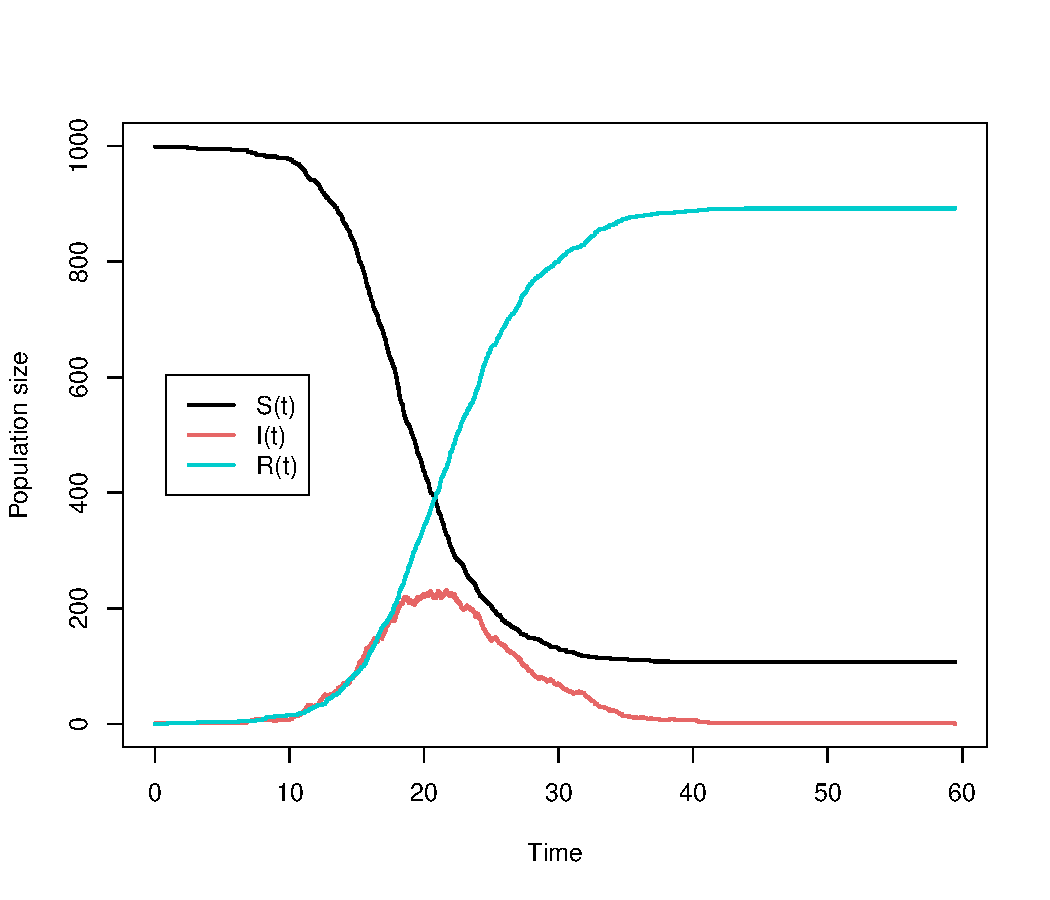
\includegraphics[width=6in]{figure1.pdf}
    \end{center}
    \caption{A single set of stochastic SIR trajectories for
      susceptible $S$, infected $I$, and recovered $R$ populations.}
	\label{fig:SIRRh_traj}
\end{figure}
%
\begin{figure}
  \begin{center}
    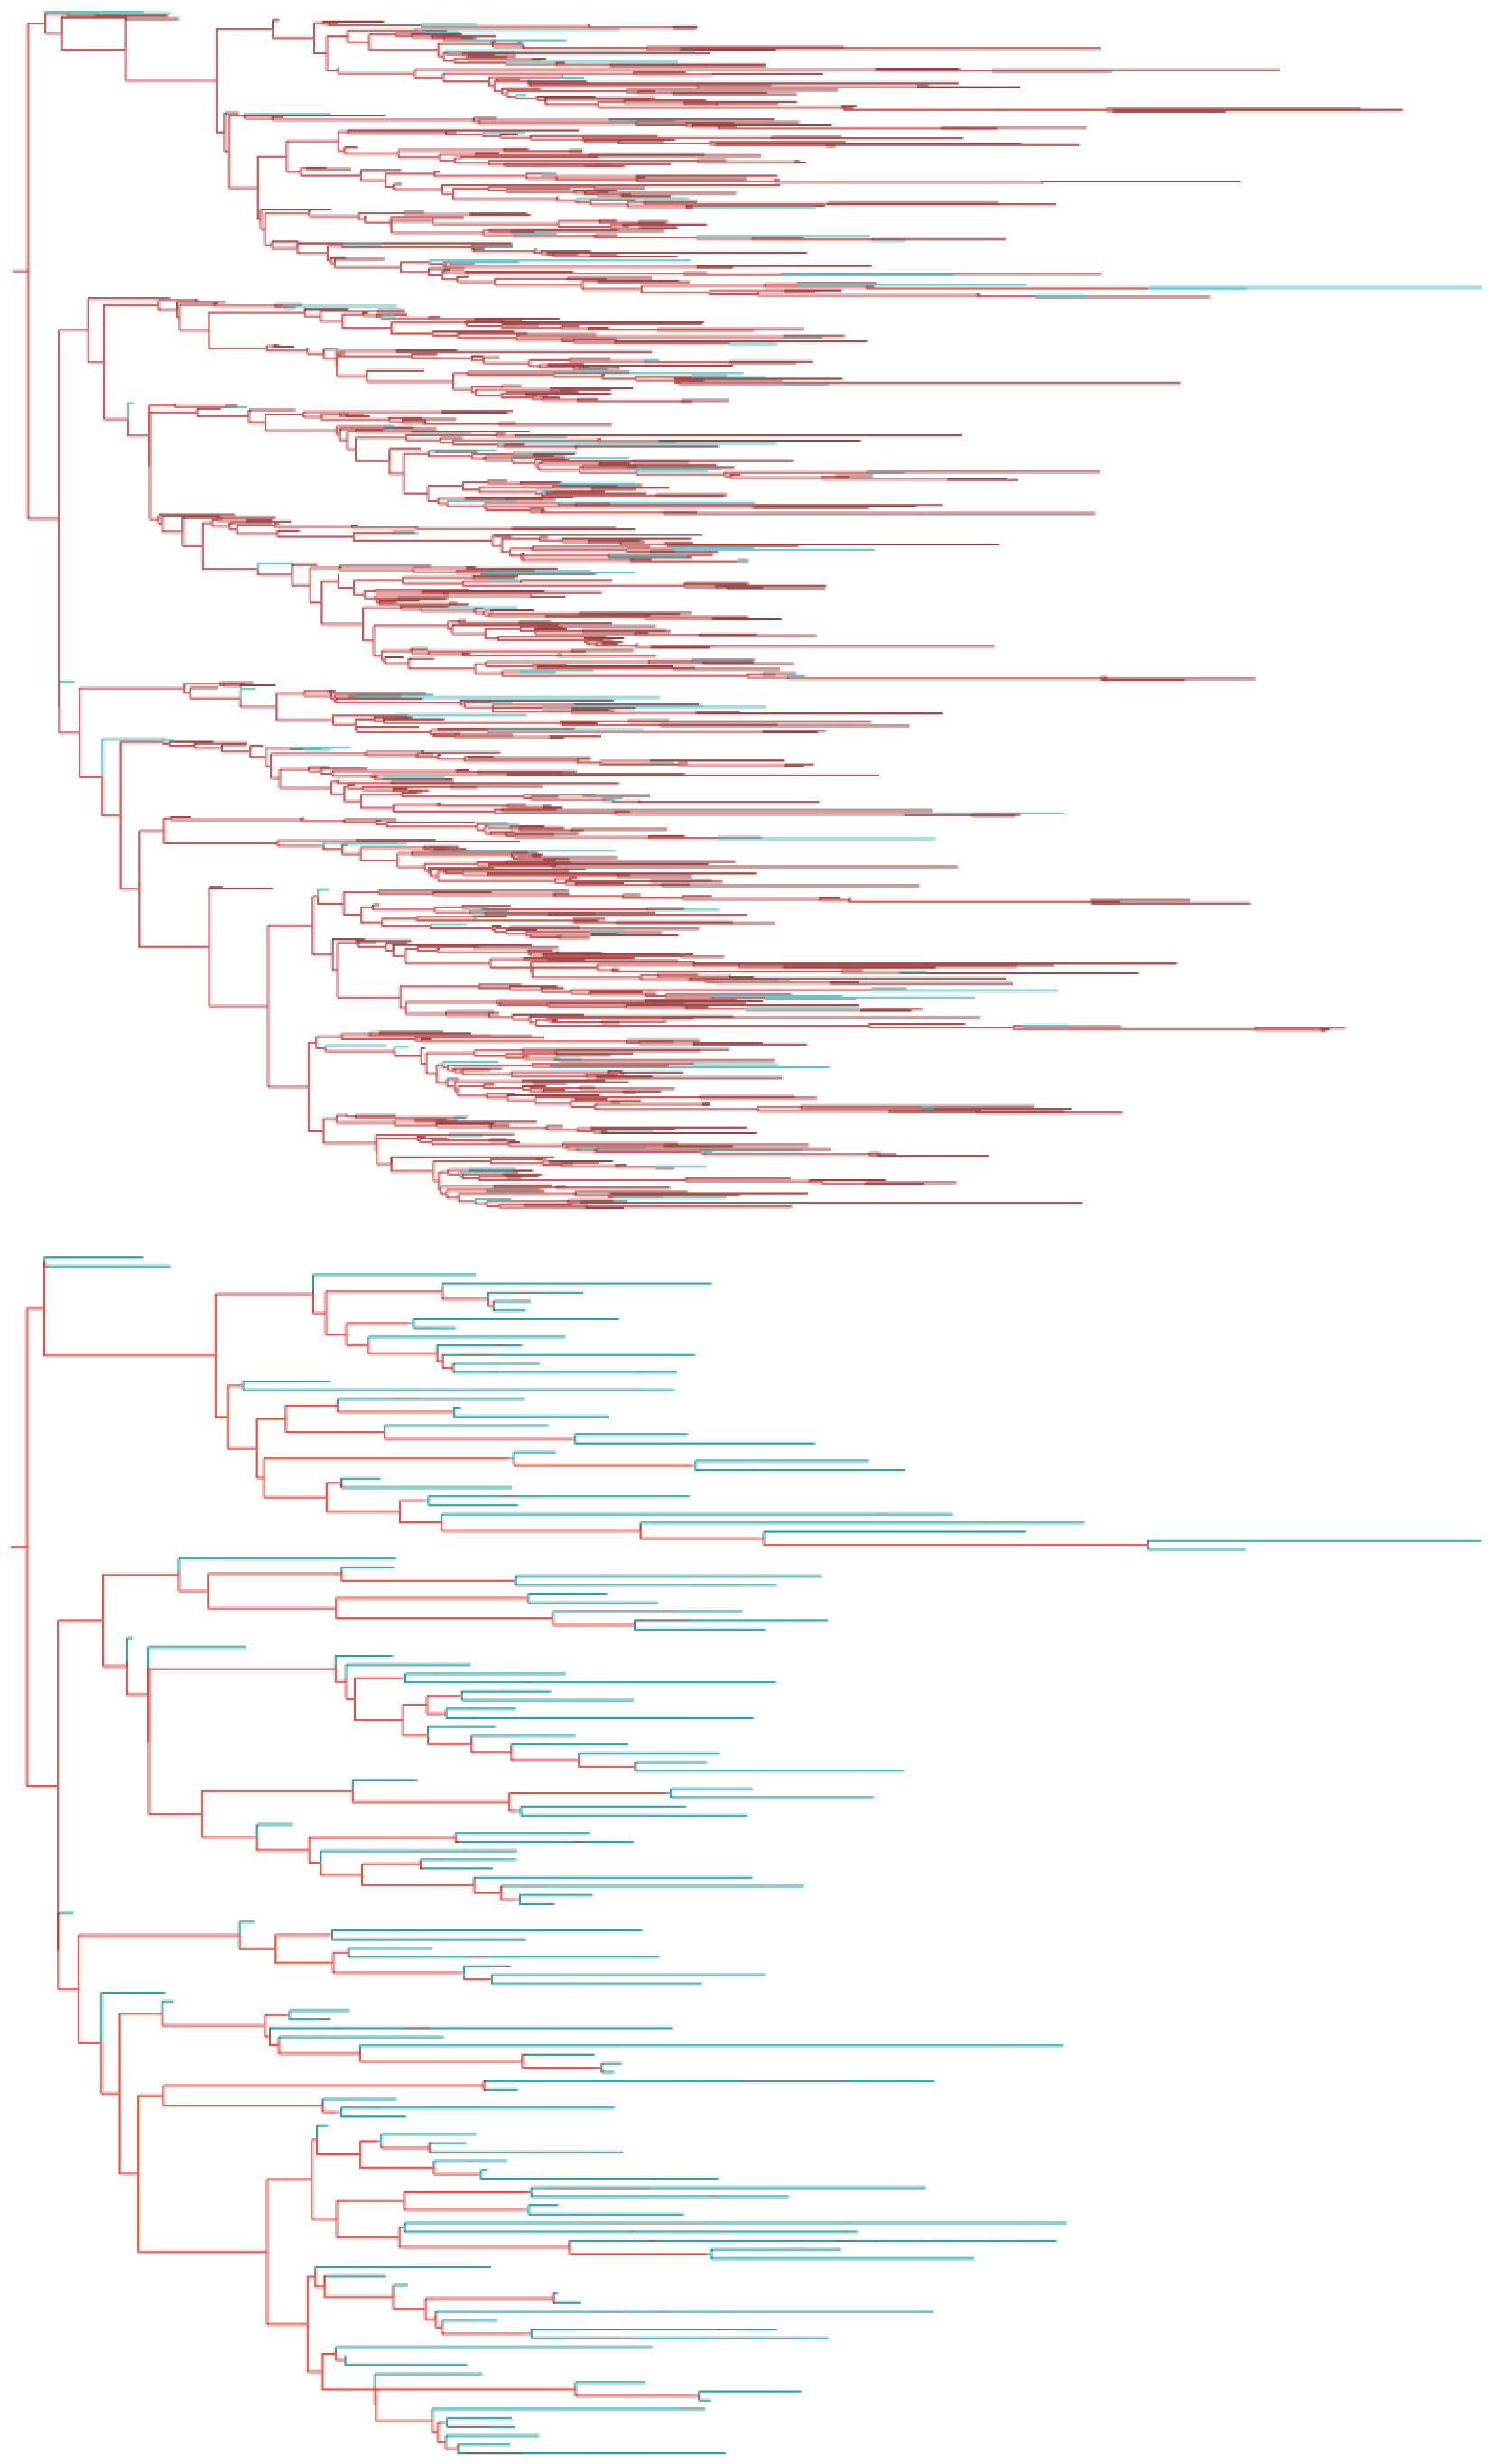
\includegraphics[width=4in]{Tree_combined.pdf}
  \end{center}
    \caption{(Top) Full tree with both sampled $\psi$ and otherwise removed $\mu$ tips. 
      (Bottom) 136-tip \textit{sampled} used as one of the 100 trees 
      (with an average of 160 tips) in the analyses of true stochastic SIR trees. 
      Figures generated by FigTree (\cite{FigTree}, 2007).}
  \label{fig:Tree}
\end{figure}
% 
\begin{figure}[ht]
    \centering
{%
    	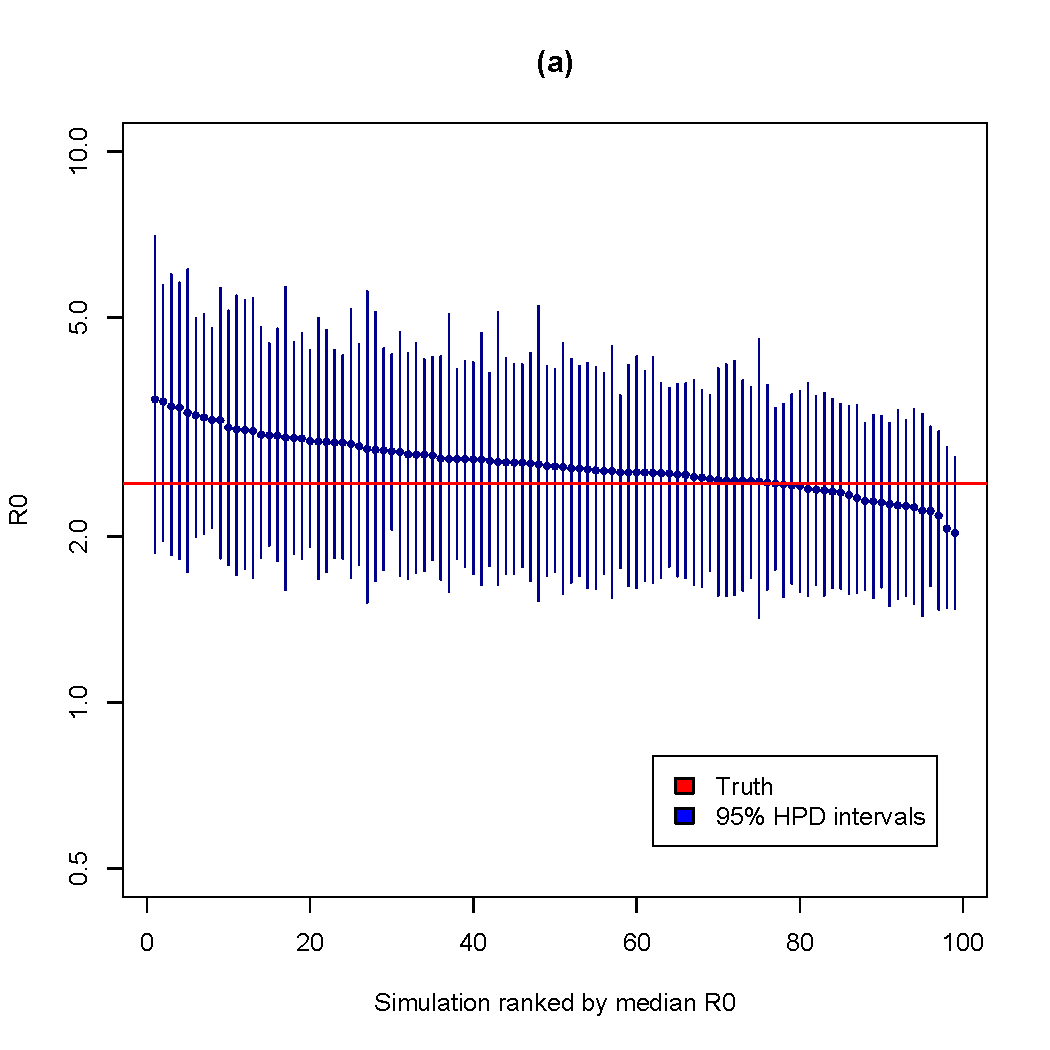
\includegraphics[width=1.99in]{R0_MASTER_stochSIR_FINAL.pdf}
}
\quad
{%
    	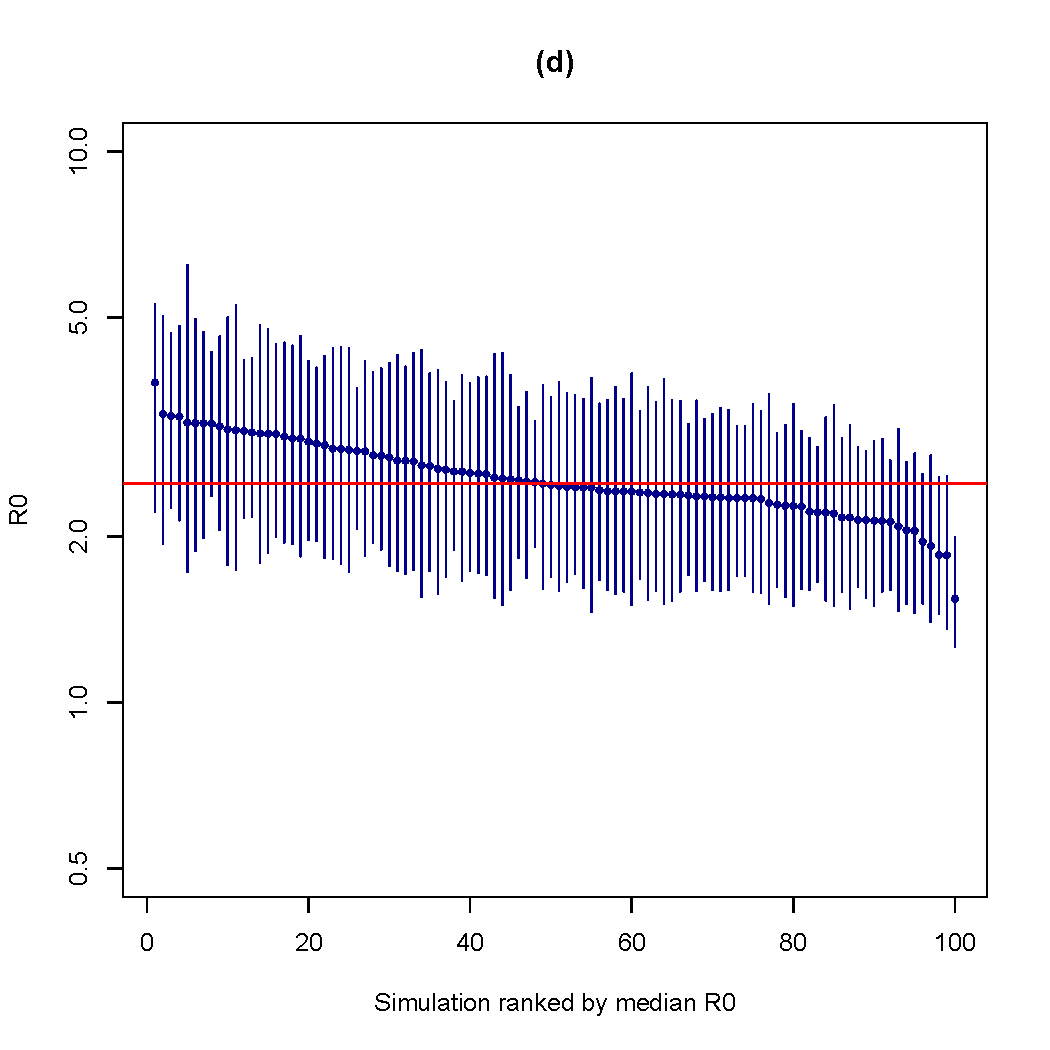
\includegraphics[width=1.99in]{R0_MASTER_deterSIR_FINAL.pdf}
}
\quad
{%
    	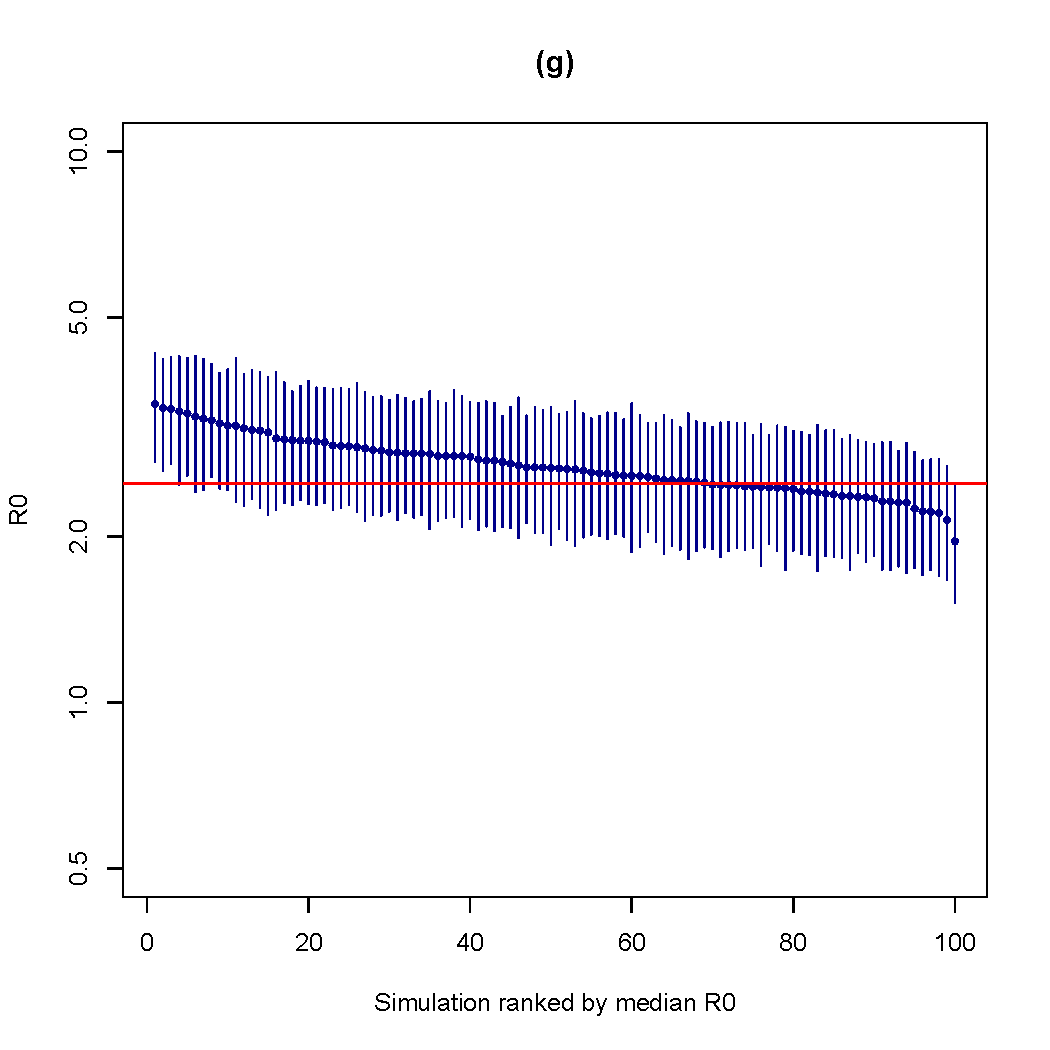
\includegraphics[width=1.99in]{R0_MASTER_BDSIR_FINAL.pdf}
}
\quad
{%
    	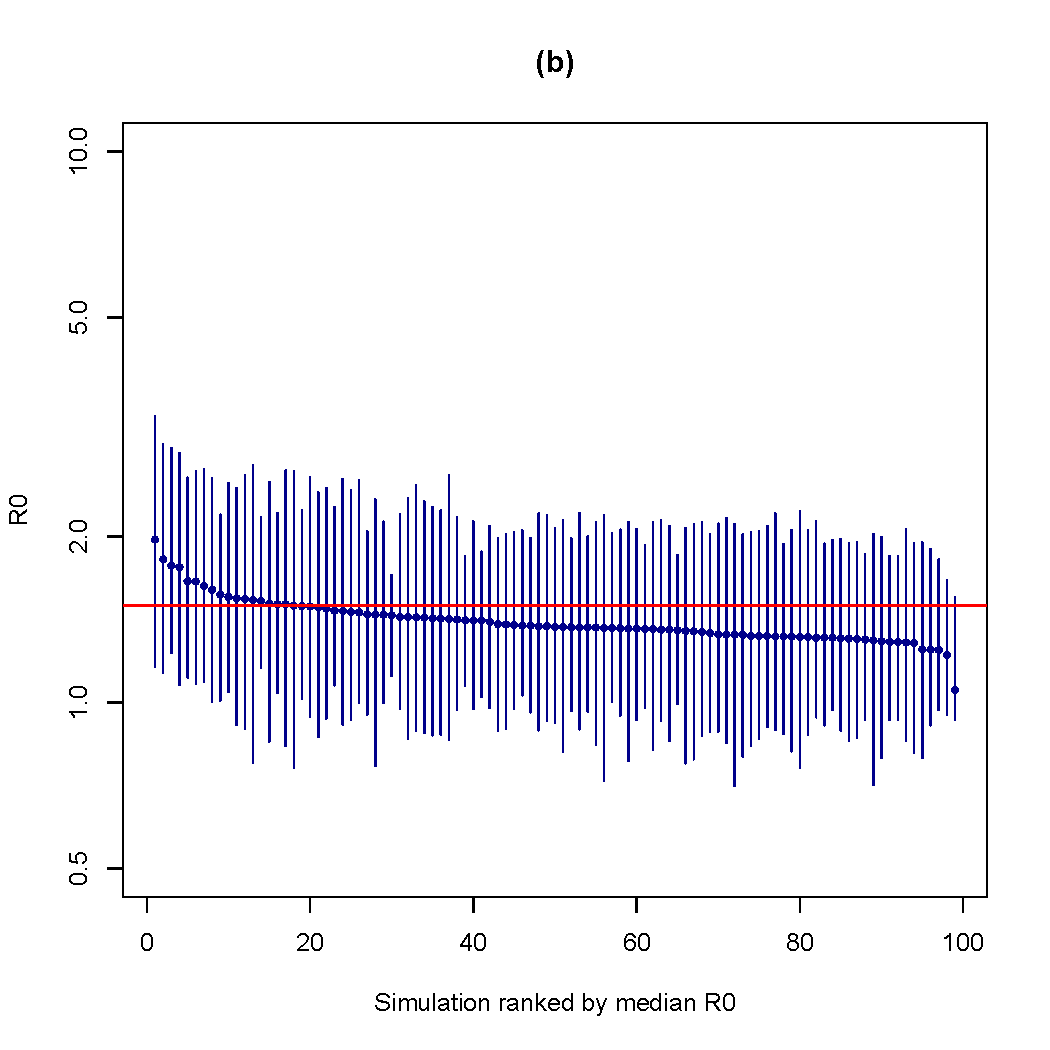
\includegraphics[width=1.99in]{R0_lowerS0_stochSIR_FINAL.pdf}
}
\quad
{%
    	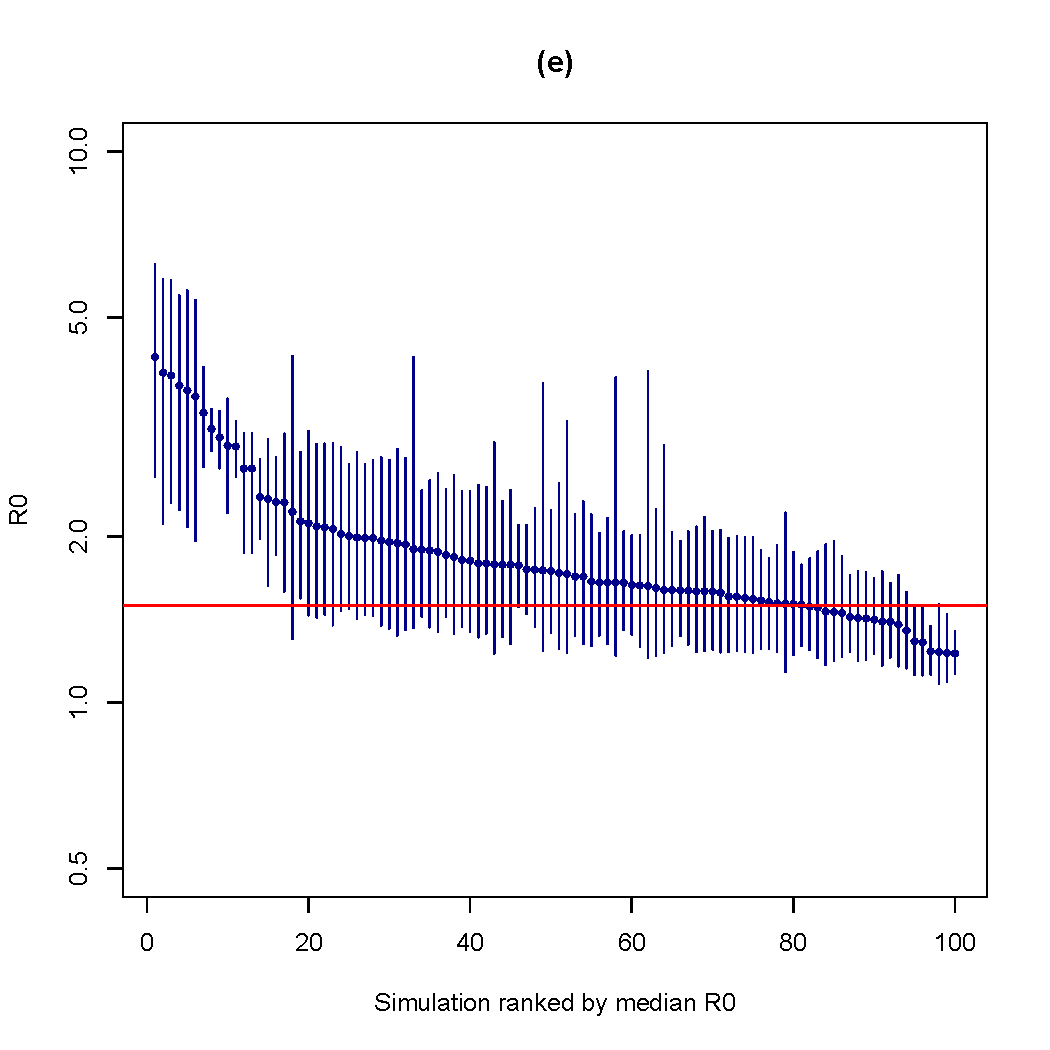
\includegraphics[width=1.99in]{R0_lowerS0_deterSIR_FINAL.pdf}
}
\quad
{%
    	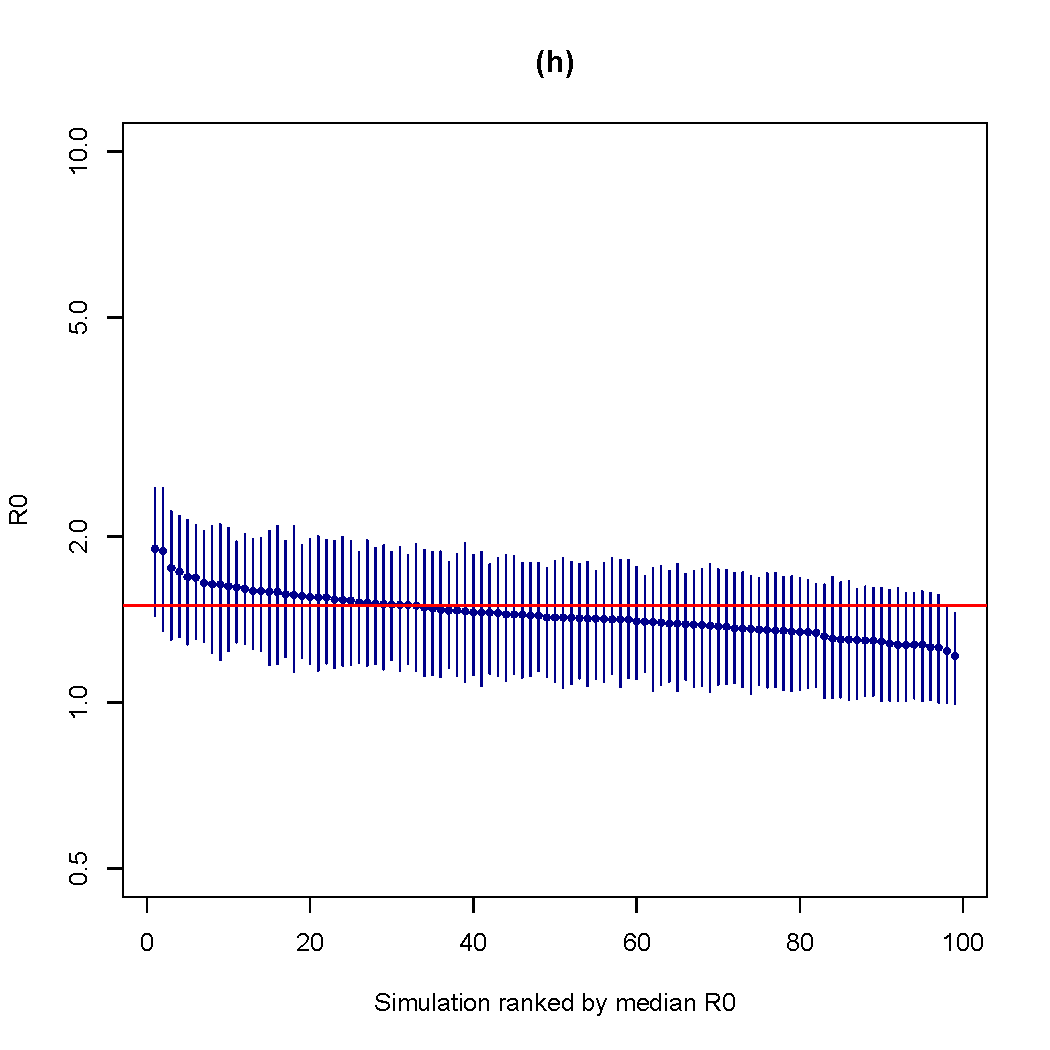
\includegraphics[width=1.99in]{R0_lowerS0_BDSIR_FINAL.pdf}
}
\quad
{%
    	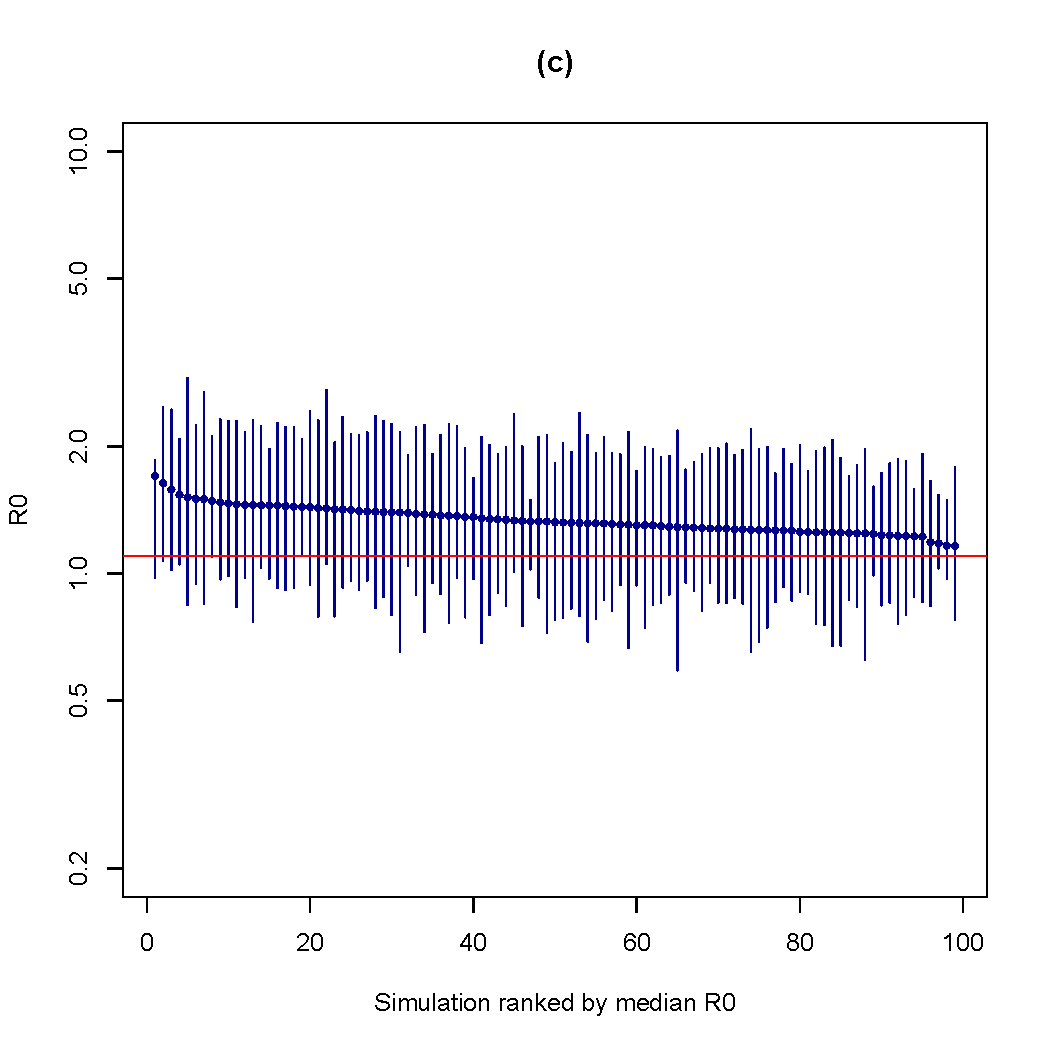
\includegraphics[width=1.99in]{R0_lowestR0_stochSIR_FINAL.pdf}
}
\quad
{%
    	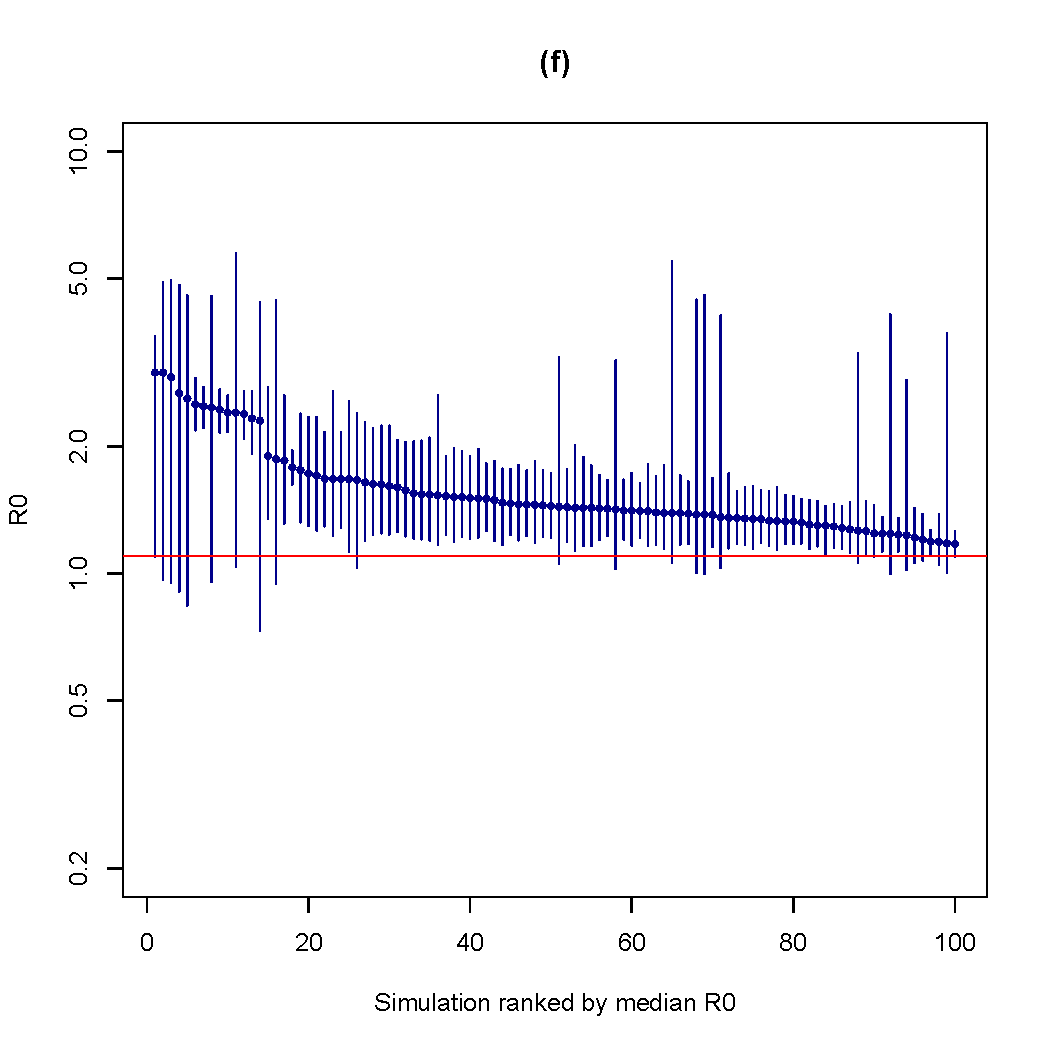
\includegraphics[width=1.99in]{R0_lowestR0_deterSIR_FINAL.pdf}
}
\quad
{%
    	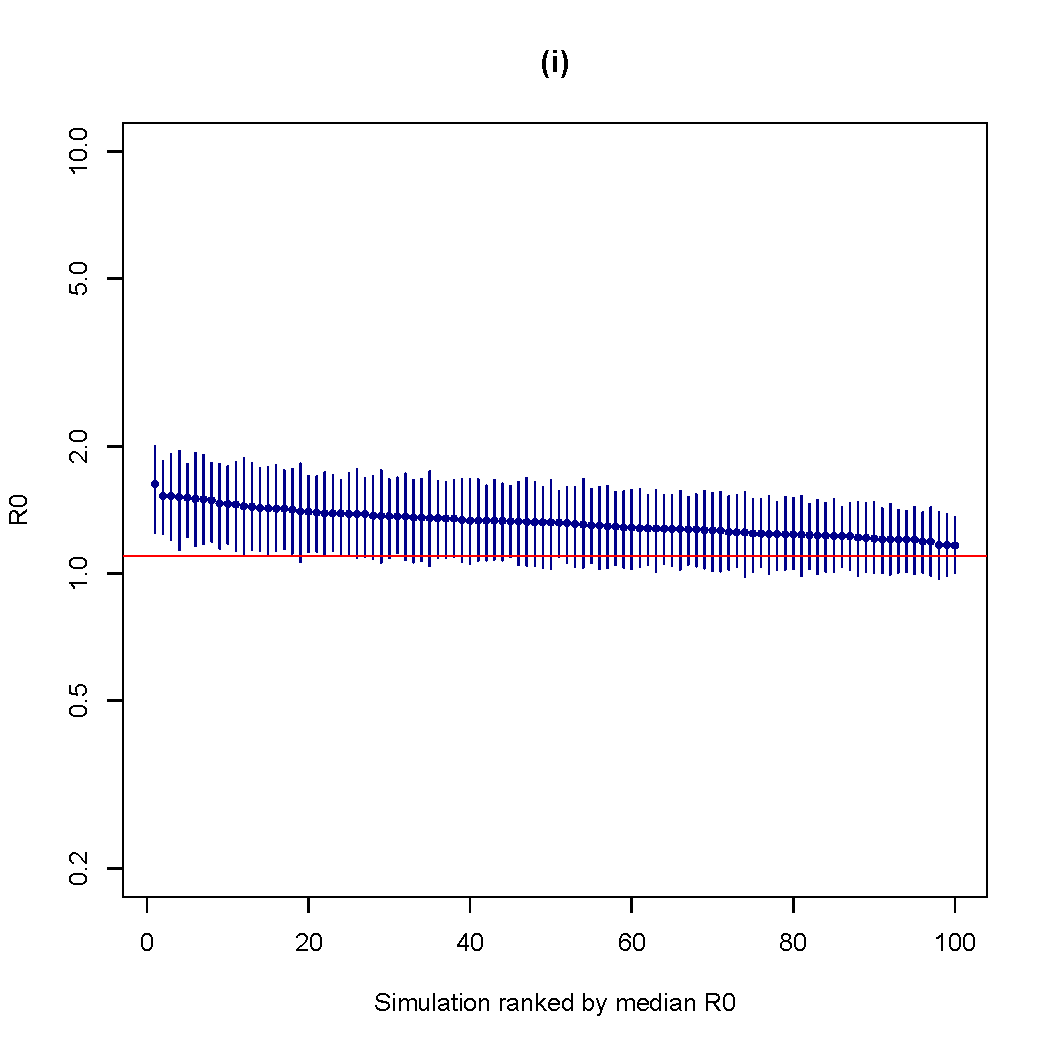
\includegraphics[width=1.99in]{R0_lowestR0_BDSIR_FINAL.pdf}
}
\caption{Estimates of $R_{(0)}$ from true stochastic SIR trees using inference methods by column, with 
	\stochCoalSIR{} (a, b, c), \deterCoalSIR{} (d, e, f), and \BDSIR{} (g, h, i).  The truth varies 
	by row, with $R_{0}=2.4975$ (a, d, g), $R_{0}=1.4970$ (b, e, h), and $R_{0}=1.0978$ (c, f, i).
}
\label{fig:blah}
\end{figure}
%
\begin{figure}[!ht]
\begin{center}
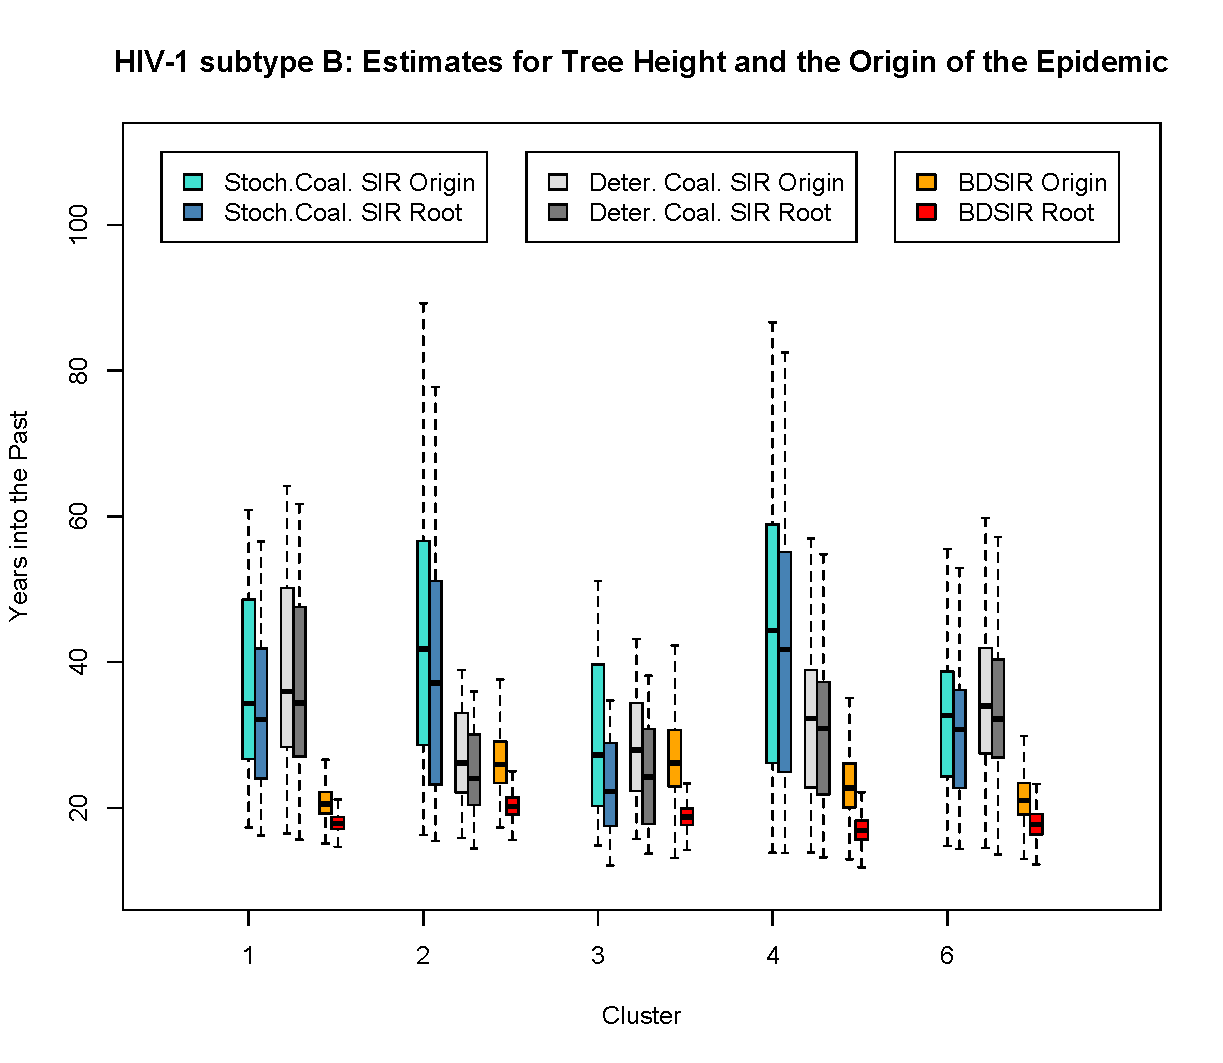
\includegraphics[width=7in]{HIV1subtypeB_treeHeight_Origin.pdf}
\end{center}
\caption{
95\% HPD intervals for coalescent [\protect\cite{Volz:2012}] and birth-death [\protect\cite{Kuhnert:2014}]
estimations of the time into the past at which the root of the HIV-1 tree and introduction 
of the first infection occurred.}
\label{fig:HIV_HeightandOrigin}
\end{figure}
%
\begin{figure}[!ht]
\begin{center}
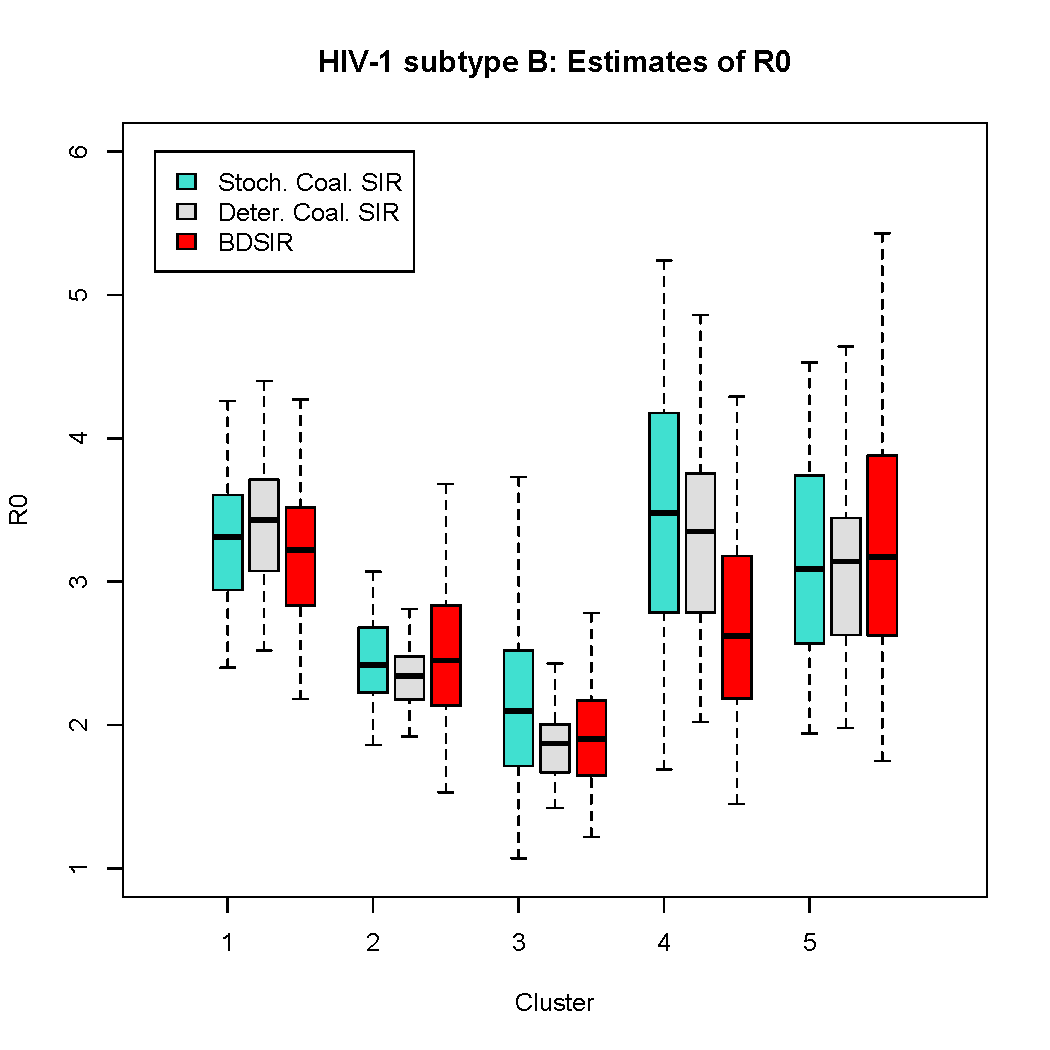
\includegraphics[width=7in]{HIV1subtypeB_R0.pdf}
\end{center}
\caption{
95\% HPD intervals of $R_0$ for the HIV-1 subtype B UK cluster 
analyses using coalescent and birth-death methods.}
\label{fig:HIV_R0}
\end{figure}
%
\begin{figure}[!ht]
\begin{center}
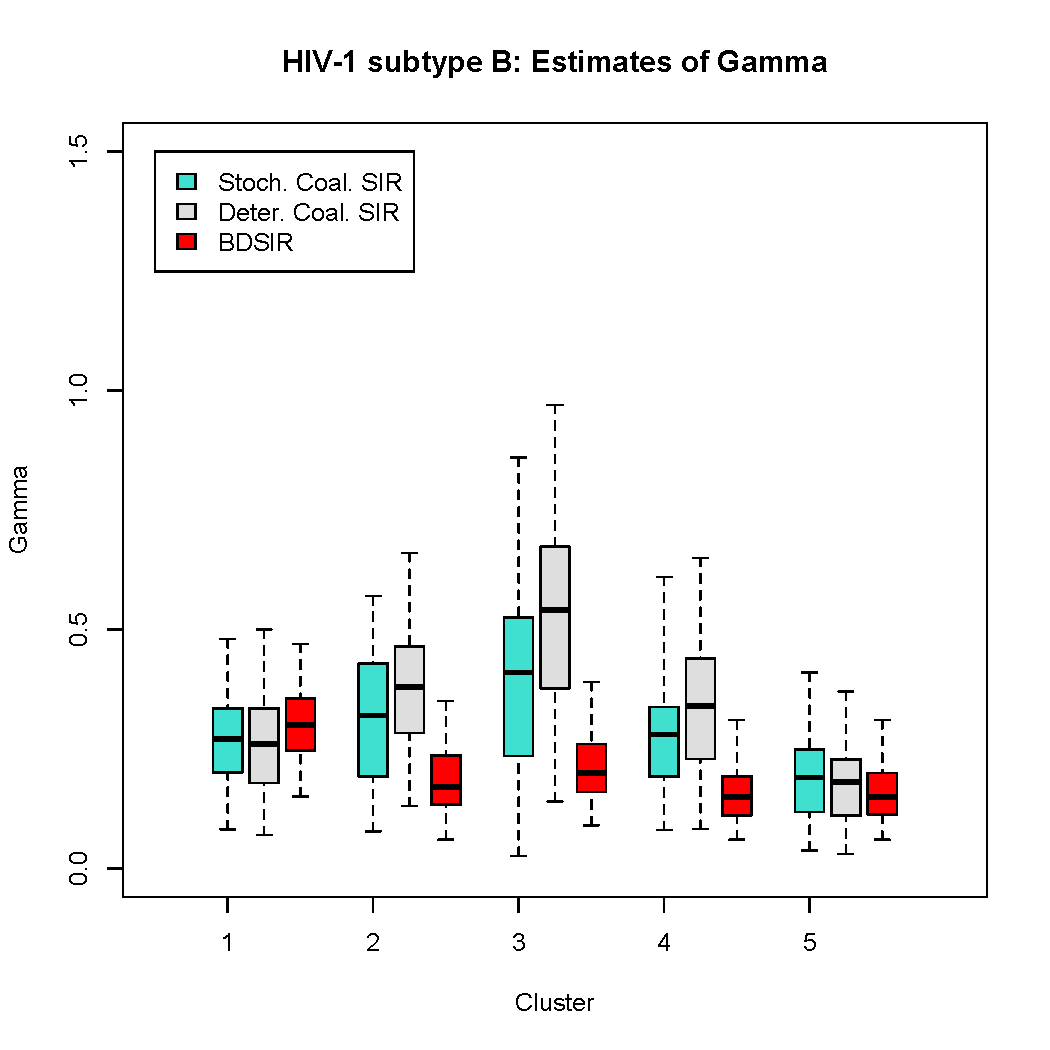
\includegraphics[width=7in]{HIV1subtypeB_gamma.pdf}
\end{center}
\caption{
95\% HPD intervals of $\gamma$ for the HIV-1 subtype B UK cluster 
analyses using coalescent and birth-death methods.}
\label{fig:HIV_gamma}
\end{figure}
%
\begin{figure}[!ht]
\begin{center}
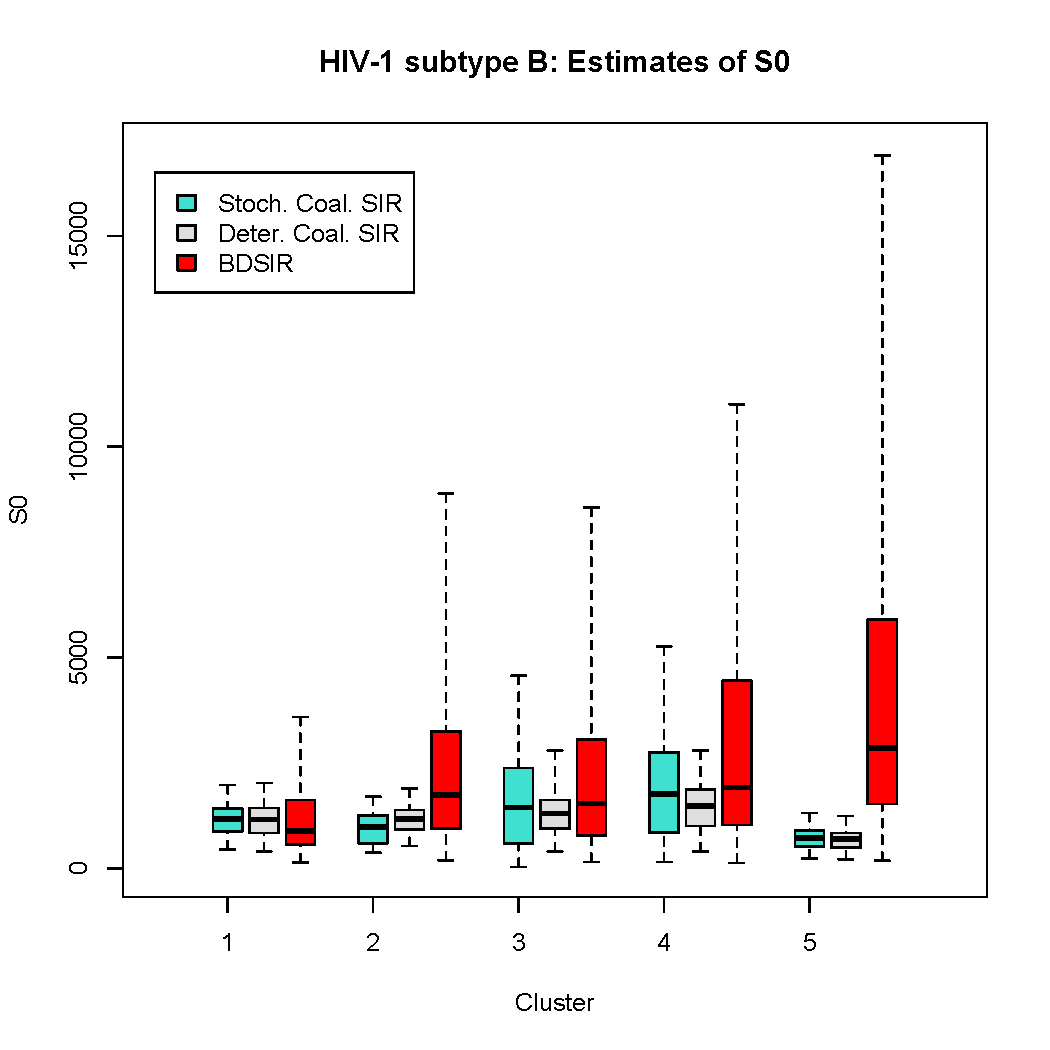
\includegraphics[width=7in]{HIV1subtypeB_S0.pdf}
\end{center}
\caption{95\% HPD intervals of $S_0$ for the HIV-1 subtype B UK cluster 
analyses using coalescent and birth-death methods.}
\label{fig:HIV_S0}
\end{figure}
%
\begin{table}[!ht]
\begin{center}
\caption{
\bf{Simulation Study Results:  $R_{0}=1.50$, $S_{0}=499$}}
\label{table:simStudy}
\begin{tabular}{|c|c|c|c|c|c|c|c|c|}
\hline
$\eta$ & Inference & Truth & Mean & Median & Error & Bias & Relative & 95\% HPD \\ 
&  &  &  &  &  &  &  HPD width & accuracy \\ 
	\hline
	\hline
& Stoch.Coal.SIR & 1.50 & 1.48 & 1.37 & 0.09 & -0.06 & 0.81 & 100.00\% \\
$\mathcal{R}_0$ & Deter.Coal.SIR & 1.50 & 1.80 & 1.49 & 0.24 & 0.15 & 0.52 & 85.00\% \\
& \BDSIR{} & 1.50 & 1.46 & 1.43 & 0.08 & -0.03 & 0.47 & 99.00\% \\ 
   \hline
   \hline 
& Stoch.Coal.SIR & 0.30 & 0.19 & 0.17 & 0.40 & -0.40 & 1.06 & 85.00\% \\
$\gamma$ & Deter.Coal.SIR  & 0.30 & 0.26 & 0.23 & 0.27 & -0.22 & 1.15 & 89.00\% \\
& \BDSIR{} & 0.30 & 0.26 & 0.25 & 0.18 & -0.18 & 0.72 & 97.00\% \\ 
   \hline
   \hline
& Stoch.Coal.SIR & 499.00 & 599.39 & 389.88 & 0.25 & -0.22 & 3.56 & 100.00\% \\
$S_{(0)}$ & Deter.Coal.SIR & 499.00 & 561.72 & 361.36 & 0.44 & -0.26 & 3.36 & 91.00\% \\
& \BDSIR{} & 499.00 & 996.12 & 713.56 & 0.51 & 0.49 & 4.63 & 100.00\% \\ 
   \hline
   \hline
& Stoch.Coal.SIR & (varies) & 76.47 & 68.24 & 0.55 & 0.54 & 0.58 & 99.00\% \\
$z_{(0)}$ & Deter.Coal.SIR & (varies) & 91.03 & 72.51 & 0.39 & 0.38 & 0.42 & 88.00\% \\
& \BDSIR{} & (varies) & 69.11 & 66.51 & 0.34 & -0.31 & 0.20 & 94.00\% \\  
   \hline
\end{tabular}
\end{center}
\end{table}
%
\begin{table}[!ht]
\begin{center}
\caption{\bf{Simulation Study:  Results for Deterministic Coalescent SIR}}
\label{table:simStudyDet}
\begin{tabular}{|c|c|c|c|c|c|c|c|c|}
\hline
$\eta$ & Inference & Truth & Mean & Median & Error & Bias & Relative & 95\% HPD \\ 
&  &  &  &  &  &  &  HPD width & accuracy \\ 
	\hline
	\hline
& Deter.Coal.SIR & 2.50 & 2.68 & 2.49 & 0.13 & 0.04 & 0.81 & 98.00\% \\
$\mathcal{R}_0$ & Deter.Coal.SIR & 1.50 & 1.96 & 1.72 & 0.30 & 0.27 & 0.62 & 80.00\% \\
& Deter.Coal.SIR & 1.20 & 1.80 & 1.49 & 0.43 & 0.43 & 0.65 & 55.00\% \\
& Deter.Coal.SIR & 1.10 & 1.68 & 1.44 & 0.46 & 0.46 & 0.59 & 25.00\% \\
   \hline
   \hline 
& Deter.Coal.SIR & 0.30 & 0.32 & 0.29 & 0.16 & 3.14\mbox{\sc{e}-3} & 1.27 & 99.00\% \\
$\gamma$ & Deter.Coal.SIR  & 0.30 & 0.26 & 0.25 & 0.25 & -0.20 & 1.04 & 90.00\% \\   
& Deter.Coal.SIR & 0.30 & 0.26 & 0.23 & 0.27 & -0.22 & 1.15 & 89.00\% \\
& Deter.Coal.SIR & 0.25 & 0.22 & 0.18 & 0.30 & -0.22 & 1.16 & 86.00\% \\
   \hline
   \hline
& Deter.Coal.SIR & 999.00 & 1807.18 & 1132.48 & 0.52 & 0.29 & 4.59 & 98.00\% \\
$S_{(0)}$ & Deter.Coal.SIR & 499.00 & 570.72 & 338.90 & 0.48 & -0.20 & 2.85 & 92.00\% \\
& Deter.Coal.SIR & 499.00 & 561.72 & 361.36 & 0.44 & -0.26 & 3.36 & 91.00\% \\
& Deter.Coal.SIR & 499.00 & 553.38 & 337.10 & 0.42 & -0.26 & 3.08 & 92.00\% \\
   \hline
   \hline
& Deter.Coal.SIR & (varies) & 41.17 & 39.99 & 0.03 & 0.01 & 0.07 & 76.00\% \\
$z_{(0)}$ & Deter.Coal.SIR & (varies) & 83.17 & 64.02 & 0.39 & 0.38 & 0.42 & 88.00\% \\
& Deter.Coal.SIR & (varies) & 91.03 & 72.51 & 0.31 & -0.29 & 0.44 & 73.00\% \\
& Deter.Coal.SIR & (varies) & 112.79 & 90.37 & 0.26 & 0.26 & 0.94 & 85.00\% \\
   \hline
\end{tabular}
\end{center}
\end{table}
 %
\begin{table}[!ht]
\footnotesize
\begin{center}
\caption{
\bf{Parameter Estimations from HIV-1 type B Sequence Data}}
\label{table:hivStudy}
\begin{tabular}{|c|c|c|c|c|c|}
  \hline
\uline{Inference Model} & $R_0$ & $\gamma$ & $S_0$ & Root of & Origin $z_{0}$ of the \\ 
HIV cluster & & & & the tree (yr) & epidemic (yr) \\
   \hline
   \hline
    & & & & &\\
\bf{\StochCoalSIR} & & & & &\\
------------------ & & & & & \\
Cluster 1 & 3.31 & 0.27 & 1165 & 1971 & 1969 \\ 
 & (2.40 - 4.26) & (8.17E-2 - 0.48) & (448 - 1974) & (1946-1987) & (1942-1986) \\
Cluster 2 & 2.42 & 0.32 & 976 & 1975 & 1972 \\ 
 & (1.86 - 3.07) & (7.72E-2 - 0.57) & (371 - 1701) & (1953 - 1988) & (1947 - 1988) \\
Cluster 3 & 2.10 & 0.41 & 1442 & 1979 & 1973 \\ 
 & (1.07 - 3.73) & (2.59\mbox{\sc{e}-2} - 0.86) & (33 - 4568) & (1959 - 1990) & (1943 - 1989) \\
Cluster 4 & 3.48 & 0.28 & 1757 & 1964 & 1961 \\ 
 & (1.69 - 5.24) & (0.08 - 0.61) & (148 - 5260) & (1922 - 1990) & (1918 - 1991) \\
Cluster 6 & 3.09 & 0.19 & 727 & 1972 & 1970 \\ 
 & (1.94 - 4.53) & (3.72\mbox{\sc{e}-2} - 0.41) & (236 - 1312) & (1950 - 1989) & (1947 - 1988) \\
   \hline
   \hline
   & & & & &\\
\bf{\DeterCoalSIR} & & & & &\\
-------------------- & & & & & \\
Cluster 1 & 3.43 & 0.26 & 1158 & 1969 & 1967 \\ 
 & (2.52 - 4.40) & (6.95E-2 - 0.50) & (397 - 2023) & (1941-1987) & (1939-1986) \\
Cluster 2 & 2.34 & 0.38 & 1163 & 1979 & 1977 \\ 
 & (1.92 - 2.81) & (0.13 - 0.66) & (530 - 1895) & (1967 - 1989) & (1964 - 1987) \\
Cluster 3 & 1.87 & 0.54 & 1298 & 1979 & 1975 \\ 
 & (1.42 - 2.43) & (0.14 - 0.97) & (399 - 2267) & (1965 - 1989) & (1960 - 1987) \\
Cluster 4 & 3.35 & 0.34 & 1479 & 1972 & 1971 \\ 
 & (2.02 - 4.86) & (8.22\mbox{\sc{e}-2} - 0.65) & (397 - 2792) & (1948 - 1990) & (1946 - 1989) \\
Cluster 6 & 3.14 & 0.18 & 693 & 1971 & 1969 \\ 
 & (1.98 - 4.64) & (2.99\mbox{\sc{e}-2} - 0.37) & (213 - 1241) & (1949 - 1989) & (1943 - 1988) \\
   \hline
   \hline
   & & & & &\\
\bf{\BDSIR{}} & & & & &\\ 
--------------- & & & & & \\
Cluster 1 & 3.22 & 0.30 & 880 & 1986 & 1983 \\ 
 & (2.18-4.27) & (0.15-0.47) & (142-3592) & (1983-1988) & (1978-1987) \\
Cluster 2 & 2.45 & 0.17 & 1745 & 1983 & 1978 \\ 
& (1.53-3.68) & (0.06-0.35) & (190-8892) & (1979-1986) & (1968-1984) \\ 
Cluster 3 & 1.90 & 0.20 & 1540 & 1985 & 1978 \\ 
 & (1.22-2.78) & (0.09-0.39) & (153-8558) & (1981-1988) & (1962-1986) \\ 
Cluster 4 & 2.62 & 0.15 & 1921 & 1987 & 1981 \\ 
 & (1.45-4.29) & (0.06-0.31) & (128-11007) & (1983-1990) & (1970-1988) \\ 
Cluster 6 & 3.17 & 0.15 & 2862 & 1986 & 1983 \\  
 & (1.73-5.43) & (0.06-0.31) & (183-16909) & (1981-1989) & (1975-1989) \\ 
   \hline
\end{tabular}
\end{center}
\end{table}
%
\begin{table}[!ht]
\begin{center}
\caption{
\bf{Bayesian prior distributions}}
\label{table:priors}
\begin{tabular}{|c|c|c|c|c|c|}
\hline
& $R_0$ & $\gamma$ & $S_{(0)}$ & $z_{(0)}$ & $\psi/(\psi+\mu)$ \\
  \hline
   & & & & & \\
High $R_{0}$ + HIV1 & LogN(1, 1) & LogN(-1, 1) & LogN(7, 1) & Unif(0, 100) & Beta(1,1) \\
   & & & & & \\
   \hline
   & & & & & \\
Moderate $R_0$ & LogN(0.5, 1) & LogN(-1, 1) & LogN(6, 1) & Unif(0, 500) & Beta(1,1) \\
   & & & & & \\
   \hline
      & & & & & \\
Low $R_0$ & LogN(0.1, 1) & LogN(-1.5, 1) & LogN(6, 1) & Unif(0, 500) & Beta(1,1) \\
   & & & & & \\
   \hline
\end{tabular}
\end{center}
{Prior distributions for the re-estimation of SIR parameters -- the reproduction ratio 
$R_0$, the rate of removal $\gamma$, the number of susceptible individuals at the start of 
the epidemic $S_{(0)}$, the time of origin $z_{(0)}$, and the sampling proportion $\psi/(\psi+\mu)$ (applicable to \BDSIR{} only) -- from the simulated trees (${R_0}\approx2.5$ and ${S_0}=999$), 
HIV-1 data analyses, then simulated trees with lower reproduction ratio and susceptibles (${R_0}\approx1.5$ and ${S_0}=499$, 
and $R_{0}\approx1.10$ and $S_{0}=499$). 
LogN($M$, $S$) is a log-normal distribution with mean $M$ and 
standard deviation $S$ in log space.}
\end{table}
%
\section{Acknowledgments}
AJD was funded by a Rutherford Discovery Fellowship from the Royal Society of New Zealand. 
AP, TV, TS and AJD were also partially supported by Marsden grant \#UOA1324 from the Royal Society of New Zealand.

(http://www.royalsociety.org.nz/programmes/funds/marsden/awards/2013-awards/).  

We would also like to thank Gabriel Leventhal and Louis Du Plessis (ETH Z\"urich) for constructive and valuable input.
%
\bibliography{volzSIR}
\bibliographystyle{genetics}

\end{document}
